% @author: Felix Hekhorn
\documentclass[
  english,		% Sprache
  a4paper,		% Papierformat
  11pt,			% Schriftgröße (default 10pt)
  %DIV=12,		% Seiteneinteilung
  DIV=12,
  titlepage,
  toc=bibnumbered,
  parskip=full,  	% Absätze (full,half,false -+*)
  headings=normal,
  BCOR=12mm,
  numbers=noenddot
]{scrartcl}
%\documentclass[a4paper,10pt]{article}
\usepackage{scrtime,scrlfile,scrpage2}

\usepackage[status=draft,inline,nomargin,marginclue]{fixme}
%\usepackage[status=final]{fixme}

\usepackage[utf8]{inputenc}
%\usepackage[ngerman]{babel} % Sprache 
\usepackage[ngerman,english,main=english]{babel} % Sprache 
\selectlanguage{english}
\usepackage{amsmath, amssymb}

%\usepackage{graphicx} % Grafiken einbinden
% The following is needed in order to make the code compatible
% with both latex/dvips and pdflatex.
\ifx\pdftexversion\undefined
\usepackage[dvips]{graphicx}
\else
\usepackage[pdftex]{graphicx}
\DeclareGraphicsRule{*}{mps}{*}{}
\fi

%\usepackage[left=2cm,right=2cm,top=2.5cm,bottom=3cm]{geometry}
\usepackage{color}
\usepackage{bbm}

\usepackage{pdflscape}
\usepackage{ulem}
\usepackage{url}
\usepackage{caption}
\usepackage{subcaption}
\usepackage{array}
\usepackage{multirow}
\usepackage{listings}
\usepackage{placeins}
\usepackage{csquotes}

\usepackage{siunitx} % SI Einheiten
\usepackage[version=3]{mhchem}
\usepackage{slashed}
\usepackage{hepnames}

%\usepackage{biblatex}
\usepackage[numbers]{natbib}
%\bibliographystyle{natdin}
%\bibliographystyle{kp}
\bibliographystyle{utphys}

\usepackage{hyperref}
%\hypersetup{colorlinks=false}
\usepackage{tabularx}

\providecommand{\abs}[1]{\left|#1\right|}
\providecommand{\VektorV}[3]{
\!\left(\!\!
\begin{array}{c}
#1 \\ #2 \\ #3
\end{array}\!\!
\right)\!
}

\providecommand{\Det}[9]{
	\begin{vmatrix}
	    #1 & #2 & #3 \\
	    #4 & #5 & #6 \\
	    #7 & #8 & #9 \\	    
	\end{vmatrix}
}

\DeclareMathOperator{\Grad}{\text{grad}}
\DeclareMathOperator{\Div}{\text{div}}
\DeclareMathOperator{\Rot}{\text{rot}}
\DeclareMathOperator{\tr}{\text{tr}}

\DeclareMathOperator{\acos}{\text{arccos}}
\DeclareMathOperator{\asin}{\text{arcsin}}
\DeclareMathOperator{\atanh}{\text{artanh}}
\DeclareMathOperator{\DiLog}{\text{Li}_2}
\DeclareMathOperator{\x}{\times}
\DeclareMathOperator{\cdt}{\!\cdot\!}
\DeclareMathOperator{\del}{\partial}
\DeclareMathOperator{\EqualClaim}{\stackrel{!}{=}}
\DeclareMathOperator{\equivals}{\mathrel{\widehat{=}}}
\providecommand{\Nabla}[0]{\vec\nabla}
\providecommand{\ex}[1]{e^{#1}}
\providecommand{\EE}[1]{\cdot 10^{#1}}
\providecommand{\FT}[1]{\mathcal{FT}\left[#1\right]}
\providecommand{\Mel}[1]{\mathcal{M}\left[#1\right]}
\providecommand{\invMel}[1]{\mathcal{M}^{-1}\left[#1\right]}

\providecommand{\dt}[0]{\Derive t}
\providecommand{\dx}[0]{\Derive x}
\providecommand{\Derive}[1]{\DeriveN{#1}{}}
\providecommand{\DeriveN}[2]{\DeriveNF {#1}{#2}{}}
\providecommand{\DeriveF}[2]{\DeriveNF {#1}{}{#2}}
\providecommand{\DeriveNF}[3]{\frac {d^{#2}#3} {d #1^{#2}}}
\providecommand{\dtP}[0]{\DeriveP t}
\providecommand{\dxP}[0]{\DeriveP x}
\providecommand{\DeriveP}[1]{\DerivePN{#1}{}}
\providecommand{\DerivePF}[2]{\DerivePNF {#1} {} {#2}}
\providecommand{\DerivePN}[2]{\DerivePNF {#1} {#2} {} }
\providecommand{\DerivePNF}[3]{\frac {\partial^{#2}#3} {\partial #1^{#2}}}
\providecommand{\DerivePMF}[3]{\frac {\partial^{2}#3} {\partial #1 \partial #2}}
\providecommand{\e}[1]{\hat{e}_{#1}}
\providecommand{\pFq}[2]{{}_{#1}F_{#2}}

\providecommand{\bra}[1]{\langle#1\rvert}
\providecommand{\ket}[1]{\lvert#1\rangle}
\providecommand{\bracket}[2]{\langle#1\vert#2\rangle}
\providecommand{\normOrd}[1]{\,:\!#1\!:\,}
\providecommand{\wContr}[3]{\contraction{}{#1}{#2}{#3}#1#2#3}

\DeclareMathOperator{\Md}{\mathcal M}
\DeclareMathOperator{\Ld}{\mathcal L}
\DeclareMathOperator{\Hd}{\mathcal H}
\DeclareMathOperator{\Nd}{\hat {\mathcal N}}
\DeclareMathOperator{\To}{\hat {\mathcal T}}

\DeclareMathOperator{\MSbar}{\overline{\text{MS}}}

\DeclareRobustCommand{\PQ}{\HepGenParticle{Q}{}{}\xspace} % heavy quark
\DeclareRobustCommand{\PaQ}{\HepGenAntiParticle{Q}{}{}\xspace} % heavy anti-quark

\def\MMa{{\texttt{Mathematica}}}
\def\HEPMath{\texttt{HEPMath}}
\def\FeynCalc{\texttt{FeynCalc}}
\def\LoopTools{\texttt{LoopTools}}
\def\QCDLoop{\texttt{QCDLoop}}


\begin{document}

\section{Introduction}
\fxerror{write intro}

\subsection{Motivation}
\fxerror{write motivation}

\subsection{Notation}
To collect all soft and collinear poles we have to calculate in $n=4+\epsilon$ dimension. Unfortunaly the extension for \textit{polarized} processes is nontrivial, because the occuring Levi-Civita tensors $\varepsilon_{\mu\nu\rho\sigma}$ and $\gamma_5$. A common choice to deal with these objects is the HVBM prescription\cite{breitenlohner1977} that keeps those two objects four dimensional at the price for splitting the full $n$ dimensional space into a $n-4$ dimensional space, called \enquote{hat-space}, and a four dimensional space (that is actually never used).

In leading order (LO) we have to consider the following processes
\begin{equation}
\Pggx(q;\sigma_q) + \Pg(k_1;\sigma_{k_1}) \rightarrow \PQ(p_1)+\PaQ(p_2)
\end{equation}
The corresponding parton structure tensor $W_{\mu\mu'}^{(0)}$ can then be written as
\fxerror{avoid all order expr?}
\begin{align}
&W_{\mu\mu'}^{(0)}(k_1,q;s,t_1,u_1,q^2;\sigma_{k_1}\sigma_{q})\nonumber\\
 &= \frac 1 2 E_\epsilon K_{\Pgg\Pg}\!\int\!\frac{d^{n-1}p_1}{2E_1(2\pi)^{n-1}}\!\int\!\frac{d^{n-1}p_2}{2E_2(2\pi)^{n-1}}\delta(p_1^2-m^2) \delta(p_2^2-m^2)\nonumber\\
 &\hspace{20pt}(2\pi)^n\delta^{(n)}(k_1+q-p_1-p_2) \Md_{\mu}^{(0)}(\sigma_{k_1})\Md_{\mu'}^{(0)}(\sigma_q)
\end{align}
where the initial $1/2$ is the initial state spin average, $K_{\Pgg\Pg}$ is the color average,
\begin{align}
E_\epsilon := \left\{\begin{array}{ll}
1/(1+\epsilon/2) &\text{unpolarized}\\
1 &\text{polarized}
\end{array}\right.
\end{align}
accounts for initial freedom in $n$ dimensions for bosons and we defined the following Mandelstam variables:
\begin{equation}
s = (q+k_1)^2, \quad t_1=t-m^2=(k_1-p_2)^2-m^2, \quad u_1 = u - m^2 = (q-p_2)^2 -m^2
\end{equation}
\begin{equation}
s' = s-q^2,\quad u_1' = u_1 - q^2
\end{equation}
\fxerror{move to LO?}
The Lorentz indices $\mu$ and $\mu'$ refer to the virtual photon that is exchanged with the scattering lepton.

By using Lorentz covariance, hermiticity, parity invariance and current conservation the parton structure tensor can be decomposed into several parts:
\begin{align}
W_{\mu\mu'}^{(0)}(k_1,q;s,t_1,u_1,q^2;\sigma_{k_1},\sigma_{q}) &= \left(-g_{\mu\mu'} + \frac{q_\mu q_{\mu'}}{q^2}\right)\frac{d^2\sigma_T(s,t_1,u_1,q^2)}{dt_1du_1} \nonumber\\
 &\hspace{20pt} +\left(k_{1,\mu}-\frac{k_1\cdot q}{q^2}q_\mu\right)\left(k_{1,\mu'}-\frac{k_1\cdot q}{q^2}q_{\mu'}\right)\left(\frac{-4q^2}{{s'}^2}\right) \nonumber\\
 &\hspace{30pt} \cdot\left(\frac{d^2\sigma_T(s,t_1,u_1,q^2)}{dt_1du_1}+\frac{d^2\sigma_L(s,t_1,u_1,q^2)}{dt_1du_1}\right)
\end{align}
\fxerror{extend}
We can then define appropiate projection operators\cite{Vogelsang:1993eg}:
\begin{align}
\mathcal P_{G,\mu\mu'} &= -g_{\mu\mu'} &b_G(\epsilon) &= \frac 1 {2(1+\epsilon/2)}\\
\mathcal P_{L,\mu\mu'} &= -\frac{4q^2}{{s'}^2} k_{1,\mu}k_{1,\mu'} &b_L(\epsilon) &= 1\\
\mathcal P_{P,\mu\mu'} &= i\varepsilon_{\mu\mu'\rho\rho'}\frac{q^{\rho}k_1^{\rho'}}{s'} &b_P(\epsilon) &= 1
\end{align}
\fxerror{justify avoidance of $\Delta$?}
\begin{align}
\frac{d^2\sigma_{k}(s,t_1,u_1,q^2)}{dt_1tu_1} &= b_k(\epsilon)\mathcal P_{k,\mu\mu'}W^{\mu\mu'}
\end{align}
with $k\in\{G,L,P\}$ denoting (here and mostly ever after) the projection type. The transverse partonic cross section $d\sigma_T$ can be reconstructed from the above definitions by using
\begin{align}
\frac{d^2\sigma_T}{dt_1du_1} &= \frac{d^2\sigma_G}{dt_1du_1} + b_G(\epsilon)\frac{d^2\sigma_L}{dt_1du_1}
\end{align}

\fxerror{explain ghosts?}

\fxerror{more}



\section{Leading Order Calculations}
In leading order we have to consider photon-gluon-fusion (PGF), that is
\begin{equation}
\Pggx(q) + \Pg(k_1) \rightarrow \PQ(p_1)+\PaQ(p_2)
\end{equation}
with two contributing diagrams depicted in figure \fxerror{todo}. The result can then be written as
\begin{equation}
\hat {\mathcal P}_{k}^{\Pgg,\mu\mu'}\hat {\mathcal P}_{k}^{\Pg}\sum_{j=1}^2\Md^{(0)}_{j,\mu}\Md^{(0)*}_{j,\mu'} = 8g^2\mu_D^{-\epsilon}e^2e_H^2 N_C C_F B_{k,QED}
\end{equation}
where $g$ and $e$ are the strong and electromagnetic coupling constants respectively, $\mu_D$ is an arbitray mass parameter introduced to keep the couplings dimensionless and $e_H$ is the magnitude of the heavy quark in units of $e$. Further $N_C$ corresponds to the gauge group $SU(N_C)$ and the color factor $C_F=(N_C^2-1)/(2N_C)$ refers to the second Casimir constant of the fundamental representation for the quarks. We then find:
\begin{align}
B_{G,QED} &= \frac{t_1}{u_1} + \frac{u_1}{t_1} + \frac{4m^2s'}{t_1u_1}\left(1-\frac{m^2s'}{t_1u_1}\right)
+\frac{2s'q^2}{t_1u_1} +\frac{2q^4}{t_1u_1} + \frac{2m^2q^2}{t_1u_1}\left(2-\frac{{s'}^2}{t_1u_1}\right)\nonumber\\
 &\hspace{20pt}+\epsilon\left\{ -1 + \frac{{s'}^2}{t_1u_1} + \frac{s'q^2}{t_1u_1} -
\frac{q^4}{t_1u_1} - \frac{m^2q^2{s'}^2}{t_1^2u_1^2} \right\} + \epsilon^2\frac{{s'}^2}{4t_1u_1}\\
B_{L,QED} &= -\frac{4q^2}{s'}\left(\frac s {s'} - \frac{m^2s'}{t_1u_1}\right)\\
B_{P,QED} &= \frac 1 2\left(\frac{t_1}{u_1}+\frac{u_1}{t_1}\right)\left(\frac{2m^2 s'}{t_1u_1}-1 - \frac{2q^2}{s'}\right)\\
B_{k,QED} &= B^{(0)}_{k,QED} + \epsilon B^{(1)}_{k,QED} + \epsilon^2 B^{(2)}_{k,QED}
\end{align}

By using eq. (\ref{eq:PartonicStructureTensor0}) we can derive the $n$-dimensional $2\rightarrow 2$ phase space
\begin{equation}
dPS_2 = \!\int\!\!\frac{d^{n}p_1}{(2\pi)^{n-1}}\frac{d^{n}p_2}{(2\pi)^{n-1}}\Theta(p_{1,0})\delta(p_1^2-m^2)\Theta(p_{2,0})\delta(p_2^2-m^2)(2\pi)^n\delta^{(n)}(k_1+q-p_1-p_2)
\end{equation}
that can be solved by using the center-of-mass system (CMS) of the incoming particles\cite{Bojak:2000eu}
\begin{align}
q &= \left(\frac {s+q^2}{2\sqrt s},0,0,-\frac{s-q^2}{2\sqrt s},\hat 0\right) &
k_1 &= \frac {s-q^2}{2\sqrt s}\left(1,0,0,1,\hat 0\right)
\end{align}
such that $q+k_1=(\sqrt s,\vec 0)$ and $k_1^2 = 0$. For the outgoing particles it follows
\begin{align}
p_1 &= \frac{\sqrt s} 2 \left(1,0,\beta\sin\theta,\beta\cos\theta,\hat 0\right)&
p_2 &= \frac{\sqrt s} 2 \left(1,0,-\beta\sin\theta,-\beta\cos\theta,\hat 0\right)
\end{align}
such that $p_1+p_2 = (\sqrt s,\vec 0)$ and $p_1^2 = p_2^2=m^2$. Finally we have to use the $n$-sphere
\begin{equation}
d^nx = \frac{2\pi^{n/2}}{\Gamma(n/2)}x^{n-1} dx= \frac{\pi^{n/2}}{\Gamma(n/2)}(x^2)^{(n-2)/2} dx^2
\end{equation}
and arrive at the well known result\cite{Laenen1993162}
\begin{align}
dPS_2 &= \frac {\delta(s'+t_1+u_1)} {2s'\Gamma((n-2)/2)(4\pi)^{(n-2)/2}}\left(\frac{(t_1u_1'-s'm^2)s' - q^2t_1^2}{s'^2}\right)^{(n-4)/2}\,dt_1du_1\\
 &= \delta(s'+t_1+u_1) h_2(n)\,dt_1 du_1\\
h_2(4+\epsilon) &= \frac {2\pi S_\epsilon} {s'\Gamma(1+\epsilon/2)}\left(\frac{(t_1u_1'-s'm^2)s' - q^2t_1^2}{s'^2}\right)^{\epsilon/2}
\end{align}
with $S_\epsilon = (4\pi)^{(-2-\epsilon/2)}$.

The final double differential LO partonic cross section can then be written as
\begin{align}
{s'}^2\frac{d^2\sigma_{k,\Pg}^{(0)}(s',t_1,u_1,q^2)}{dt_1du_1} &= 2^6\alpha\alpha_s e_H^2 K_{\Pg\Pgg}N_CC_F E_k(\epsilon) b_k(\epsilon)\delta(s'+t_1+u_1) \frac{\pi^3S_\epsilon}{\Gamma(1+\epsilon/2)}  \nonumber\\
 &\hspace{20pt} \left(\frac{(t_1u_1'-s'm^2)s' - q^2t_1^2}{m^2{s'}^2}\right)^{\epsilon/2}\left(\frac{\mu_D^2}{m^2}\right)^{-\epsilon/2} B_{k,QED}
\end{align}
where we used $e^2=4\pi\alpha$ and $g^2=4\pi\alpha_s$. The color average is given by $K_{\Pg\Pgg} = 1/(N_C^2-1)$.

From the results above we can easily obtain the \textit{total} LO partonic cross sections
\begin{align}
\sigma_G^{(0)}(s,q^2,m^2) &=-4\pi\alpha\alpha_s e_H^2 K_{\Pg\Pgg}N_CC_F\frac 1 {{s'}^3}\left((s^2+q^4+4m^2 s)\beta + (s^2+q^4-4m^2(2m^2-s'))\ln(\chi)\right)\\
\sigma_L^{(0)}(s,q^2,m^2) &=16\pi\alpha\alpha_s e_H^2 K_{\Pg\Pgg}N_CC_F\left(\frac{-q^2s}{{s'}^3}\right)\left(\beta + \frac{2m^2}{s}\ln(\chi)\right)\\
\sigma_P^{(0)}(s,q^2,m^2) &=4\pi\alpha\alpha_s e_H^2 K_{\Pg\Pgg}N_CC_F\frac 1 {{s'}^2}\left((3s+q^2)\beta + (s+q^2)\ln(\chi)\right)
\end{align}
from which we also find
\begin{align}
\lim_{s\rightarrow 4m^2} \sigma_T^{(0)}(s',q^2) &= 4\pi\alpha\alpha_s e_H^2 K_{\Pg\Pgg}N_CC_F\frac{\beta}{4m^2-q^2} + O(\beta^3) = \lim_{s\rightarrow 4m^2} \sigma_P^{(0)}(s',q^2)\\
\lim_{s\rightarrow 4m^2} \sigma_L^{(0)}(s',q^2) &= -\frac{128}{3}\pi\alpha\alpha_s e_H^2 K_{\Pg\Pgg}N_CC_F\frac{m^2q^2\beta^3}{(4m^2-q^2)^3} + O(\beta^5)
\end{align}
(Note the missing factor of 2 in \cite[eq. (5.9)]{Laenen1993162}.)
\fxerror{shift to partonic?}


\section{Next-To-Leading Order Calculations}
Next-to-leading order contributions can be split into three parts: one loop virtual contributions, one gluon radiation and the light quark processes.
\fxerror{more?}

\subsection{One Loop Virtual Contributions}

\begin{align}
M_{\vec k}^{(1),V}&=\hat {\mathcal P}_{\vec k}^{\Pgg,\mu\mu'}\hat {\mathcal P}_{\vec k}^{\Pg}\sum_{j}\left[\Md^{(1),V}_{j,\mu}\left(\Md^{(0)}_{1,\mu'}+\Md^{(0)}_{2,\mu'}\right)^*+c.c.\right] \nonumber\\
 &= 8g^4\mu_D^{-\epsilon}e^2e_H^2 N_C C_FC_\epsilon\left( C_A V_{\vec k,OK} + 2C_F V_{\vec k,QED}\right)
\end{align}
where $C_\epsilon = \exp(\epsilon/2(\gamma_E-\ln(4\pi)))/(16\pi^2)$ and $C_A$ is the second Casimir constant of the adjoint representation for the gluon (that introduces a non-abelian part).

As the short example above shows, the full expressions for the $V_{k,OK},V_{k,QED}$ are quite complicated and too long to be presented here, nevertheless the arising poles are quite compact:
\begin{align}
V_{\vec k,OK} &= -2B_{\vec k,QED}\left(\frac 4 {\epsilon^2} + \left(\ln(-t_1/m^2) + \ln(-u_1/m^2) -\frac{2m^2-s}{s}\ln(\chi)\right)\frac 2 \epsilon \right) + O(\epsilon^0)\\
V_{\vec k,QED} &= -2B_{\vec k,QED}\left(1+\frac{2m^2-s}{s}\ln(\chi)\right)\frac 2 \epsilon + O(\epsilon^0)
\end{align}
The above results already include the mass renormalization that we have performed \textit{on-shell}, so all ultra-violet poles have been removed. For the renormalization of the strong coupling we use the $\MSbar_m$ scheme defined in \cite{Bojak:2000eu} and so the full (remaining) renormalization can be achieved by
\begin{align}
\frac{d^2\sigma_{\vec k}^{(1),V,ren.}}{dt_1du_1} &=\frac{d^2\sigma_{\vec k}^{(1),V}}{dt_1du_1} + \frac{\alpha_s(\mu_R^2)}{4\pi}\left[\left(\frac 2 \epsilon + \gamma_E-\ln(4\pi)+\ln(\mu_R^2/m^2)-\ln(\mu_D^2/m^2)\right)\beta_0^f \right.\nonumber\\
 &\hspace{120pt}\left.+\frac 2 3 \ln(\mu_R^2/m^2)\right]\frac{d^2\sigma_{\vec k}^{(0)}}{dt_1du_1}\\
&=\frac{d^2\sigma_{\vec k}^{(1),V}}{dt_1du_1} + 4\pi\alpha_s(\mu_R^2)C_\epsilon\left(\frac{\mu_D^2}{m^2}\right)^{-\epsilon/2}\left[\left(\frac 2 \epsilon +\ln(\mu_R^2/m^2)\right)\beta_0^f \right.\nonumber\\
 &\hspace{180pt}\left.+\frac 2 3 \ln(\mu_R^2/m^2)\right]\frac{d^2\sigma_{\vec k}^{(0)}}{dt_1du_1}
\end{align}
with $\mu_R$ the renormalization scale introduced by the RGE, $\beta_0^f = (11C_A- 2n_{f})/3$ the first coefficient of the beta function and $n_f$ the number of \textit{total} flavours (i.e. $n_{lf}=n_f-1$ active (light) flavours and one heavy flavour). The double poles occuring in $V_{\vec k,OK}$ are introduced by the diagrams \fxerror{do} when the soft and collinear singularities coincide.

The partonic cross section is given by
\begin{align}
d\sigma_{\vec k,\Pg}^{(1),V} &= \frac 1 {2s'}\frac 1 2 E_{k_2}(\epsilon) M_{\vec k}^{(1),V} dPS_2
\end{align}



\subsection{Single Gluon Radiation}
\label{sec:NLO.g}
In next-to-leading order we have to consider the following process:
\begin{equation}
\Pggx(q) + \Pg(k_1) \rightarrow \PQ(p_1)+\PaQ(p_2) + \Pg(k_2)
\end{equation}
where all contributing diagrams are depicted in figure \ref{fig:FeynNLOg}.
\begin{figure}[ht!]
\centering
\begin{subfigure}[t]{.23\textwidth}
	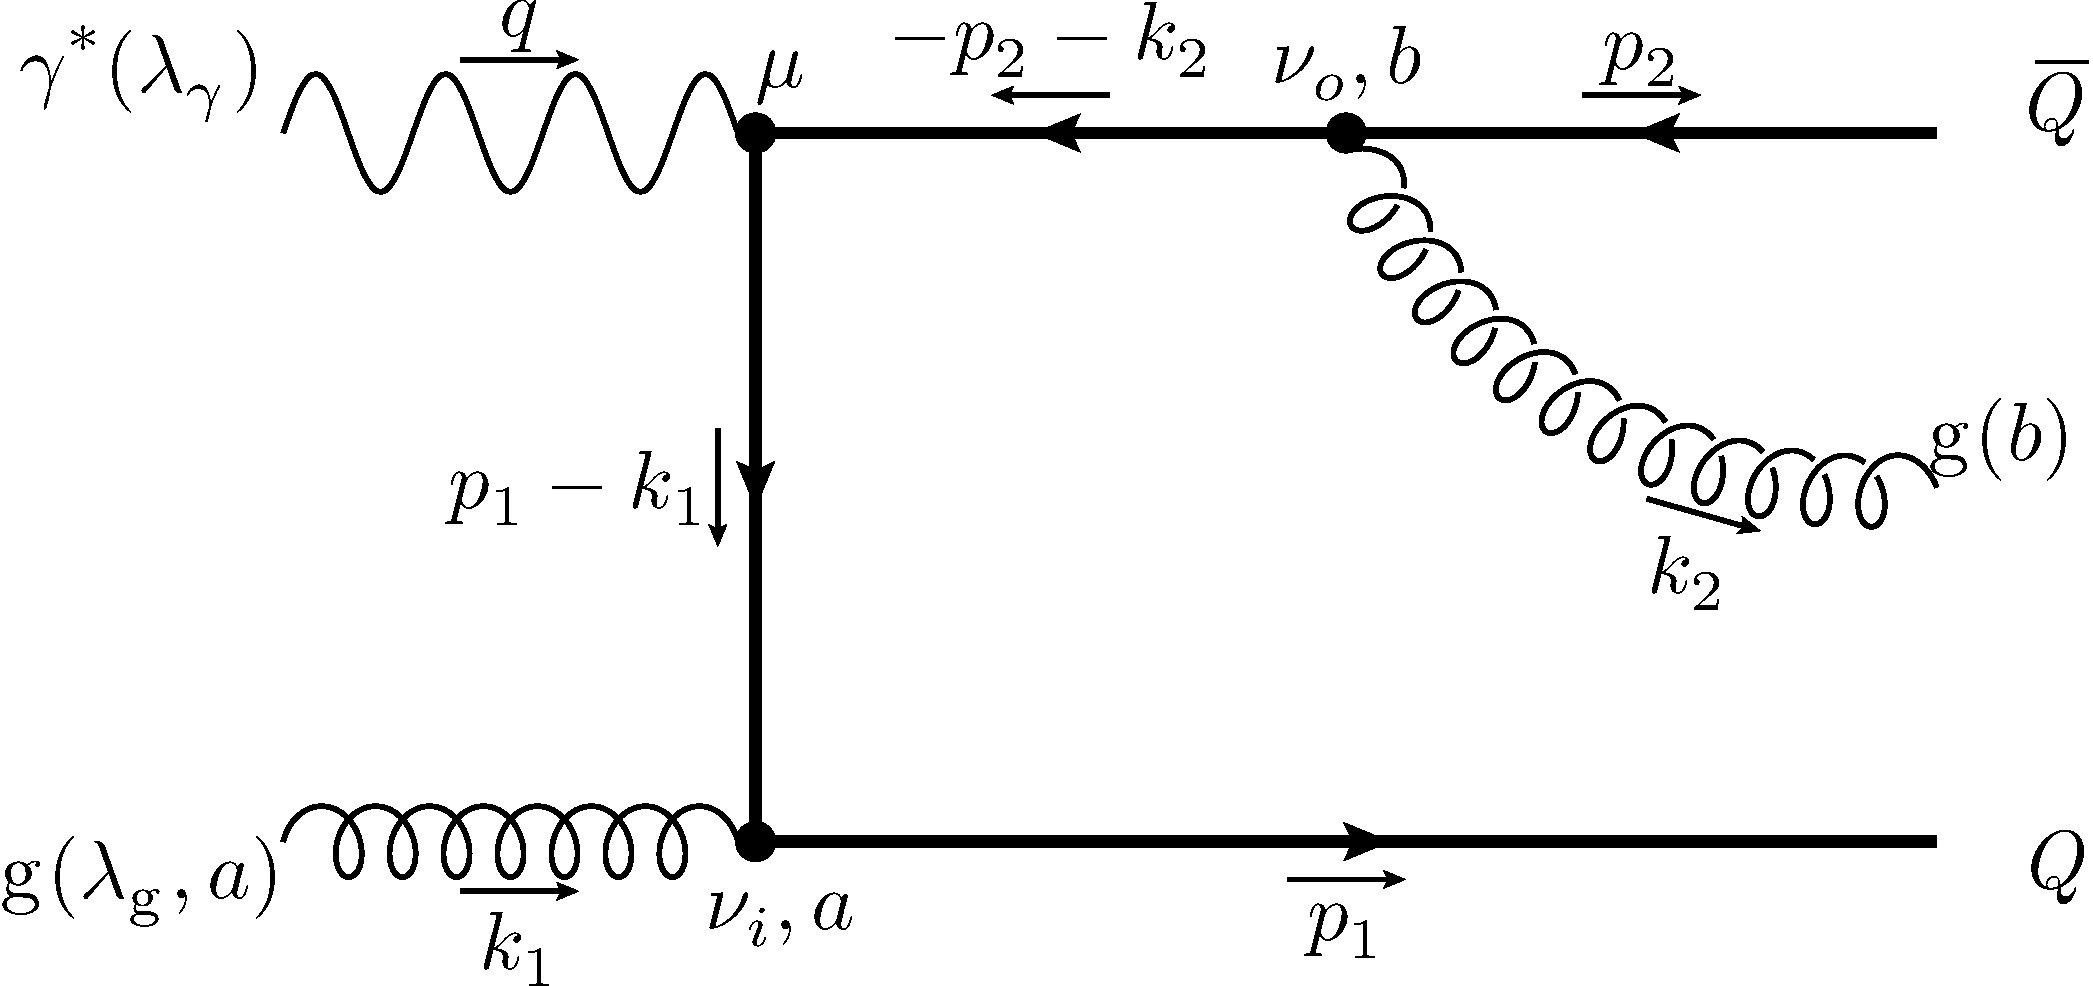
\includegraphics[width=\textwidth]{pyfeyn/nlo-g-1}
	\caption{}
\end{subfigure}\hspace{.02\textwidth}%
\begin{subfigure}[t]{.23\textwidth}
	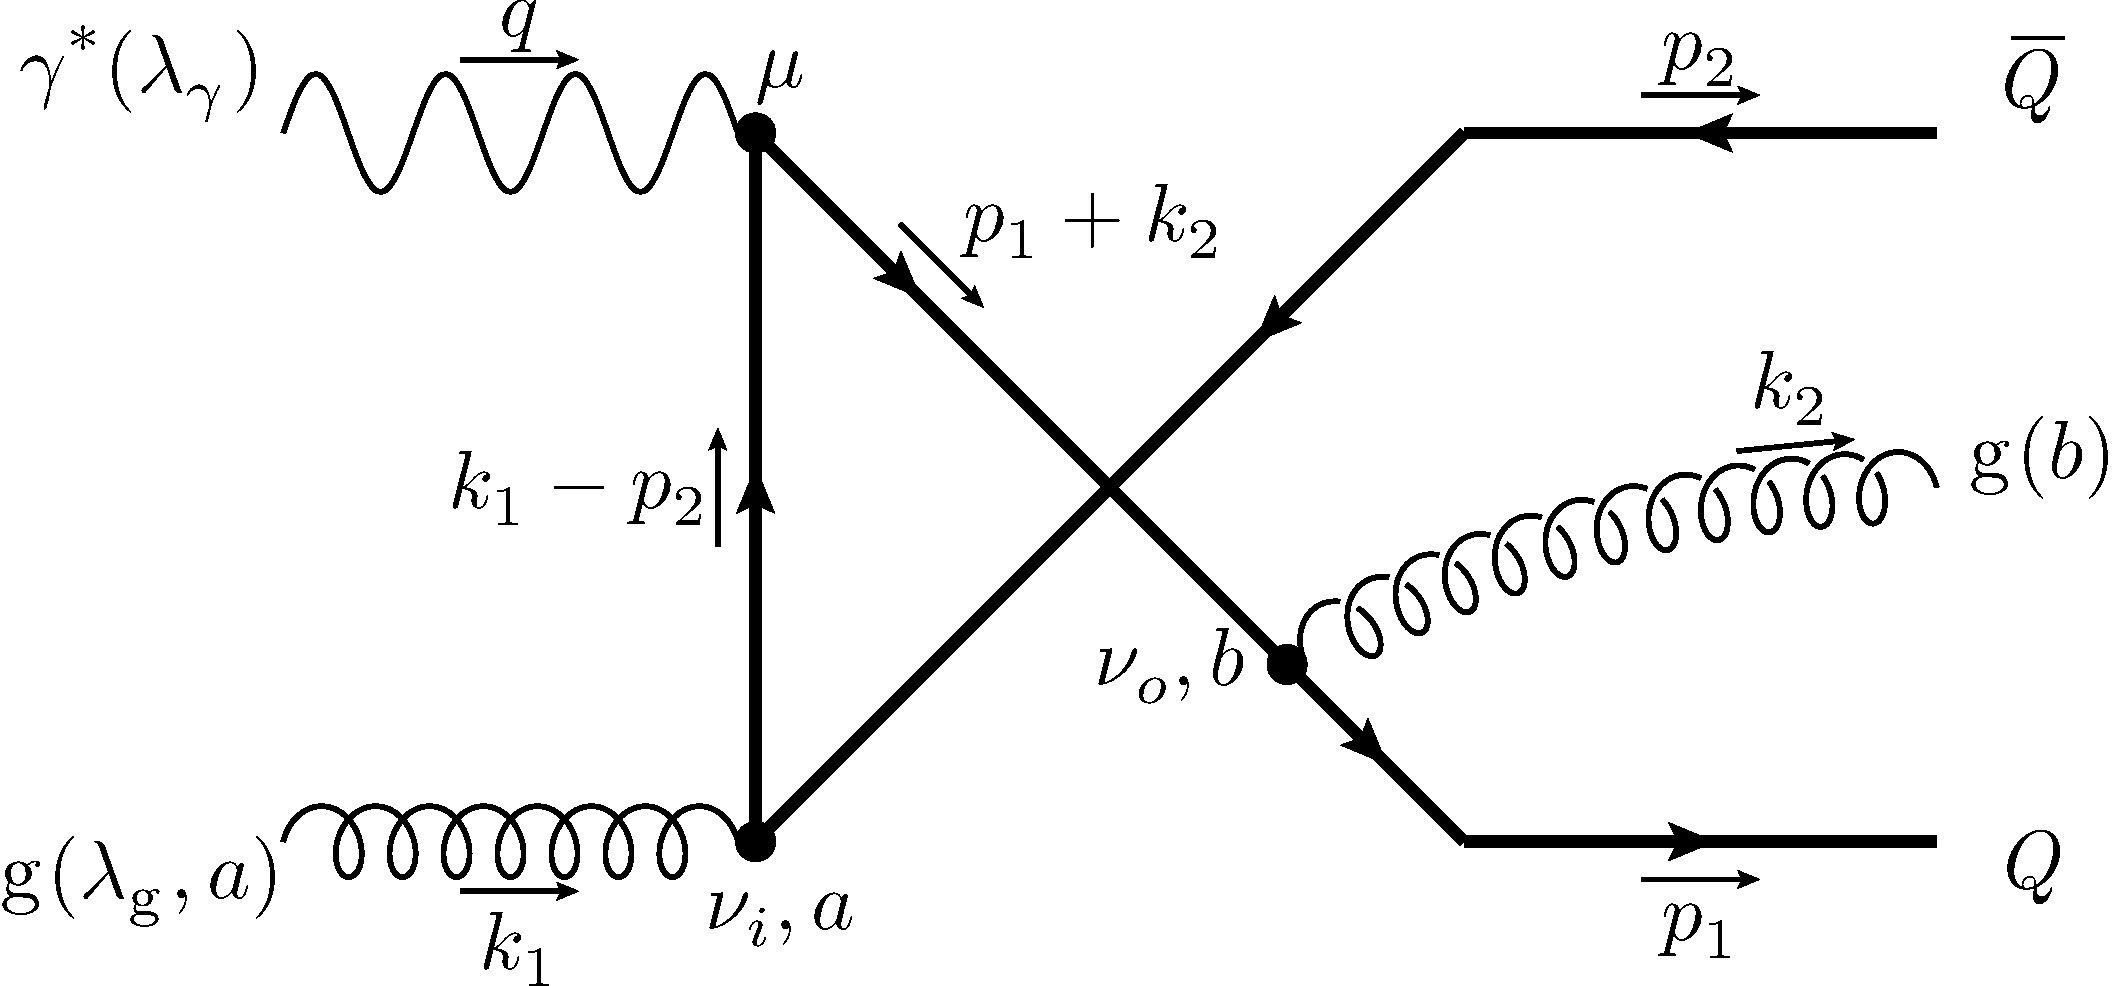
\includegraphics[width=\textwidth]{pyfeyn/nlo-g-2}
	\caption{}
\end{subfigure}\hspace{.02\textwidth}%
\begin{subfigure}[t]{.23\textwidth}
	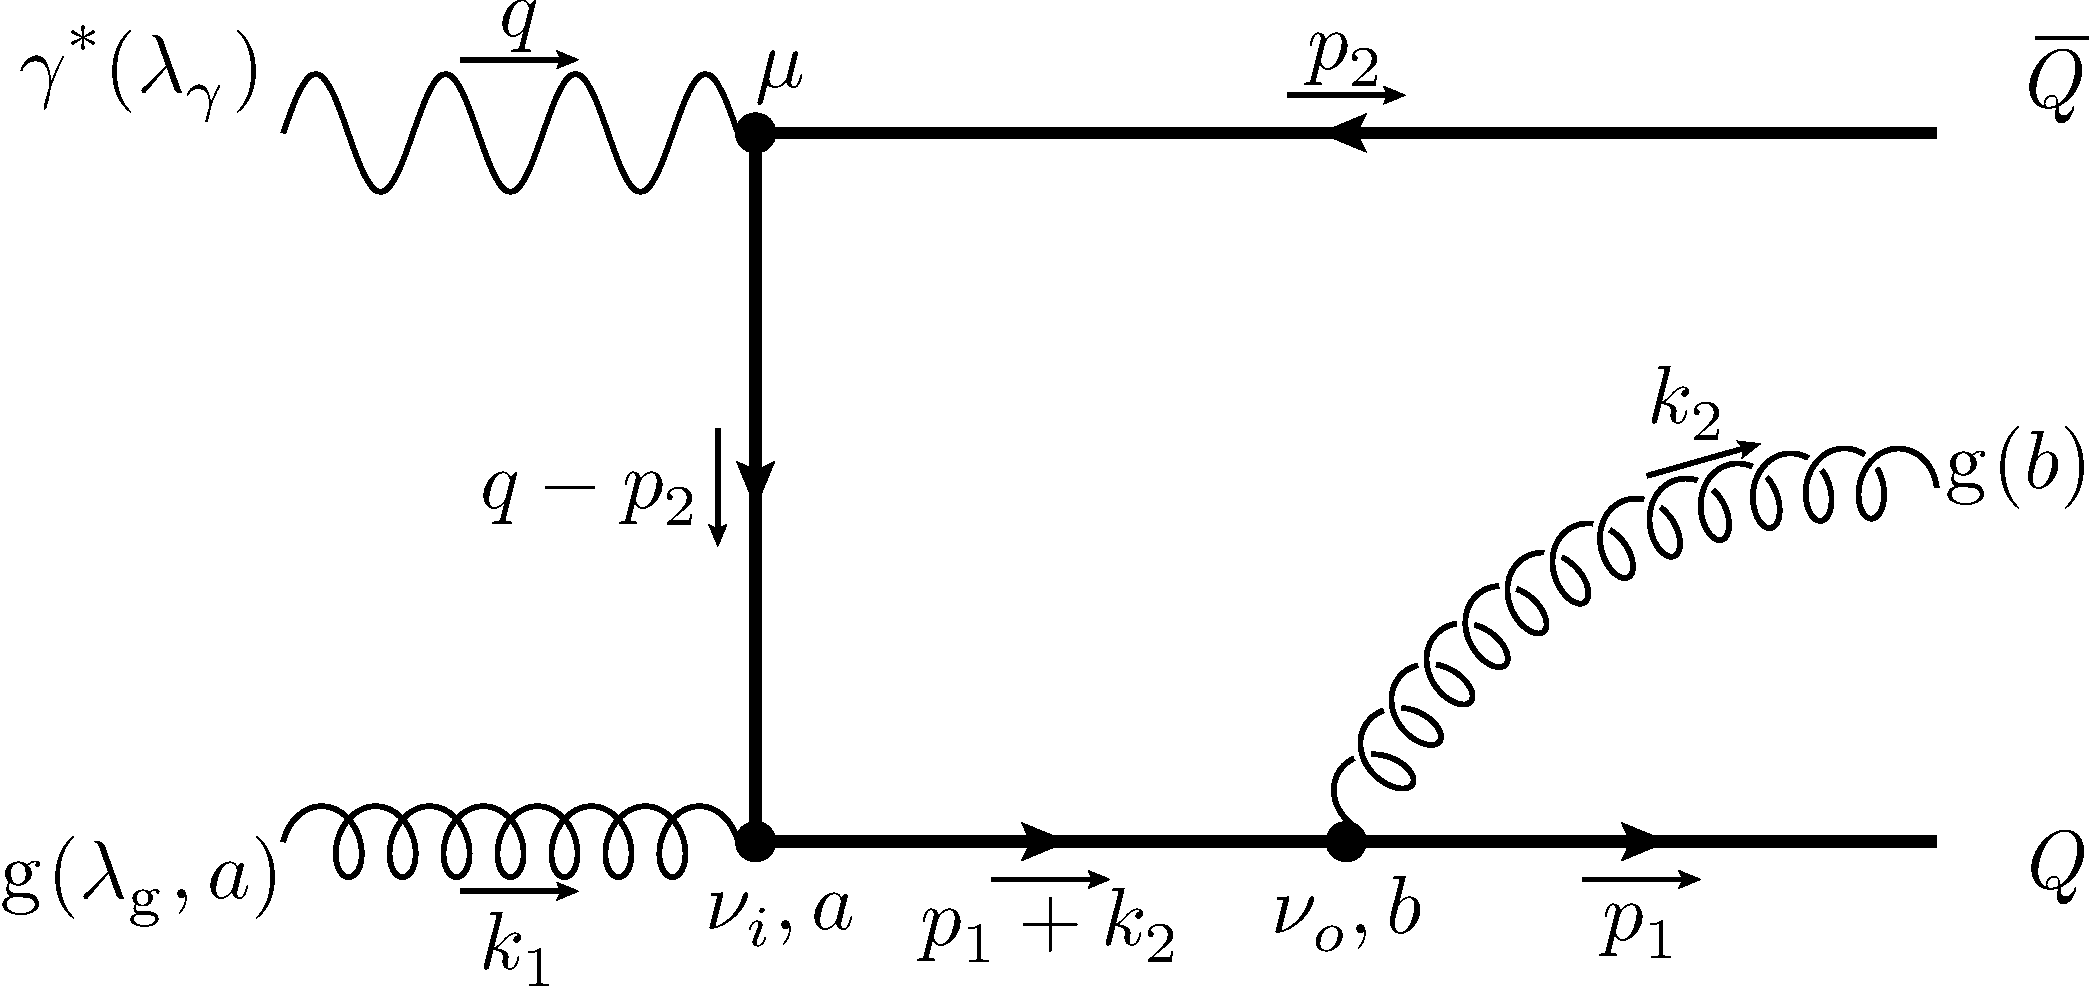
\includegraphics[width=\textwidth]{pyfeyn/nlo-g-3}
	\caption{}
\end{subfigure}\hspace{.02\textwidth}%
\begin{subfigure}[t]{.23\textwidth}
	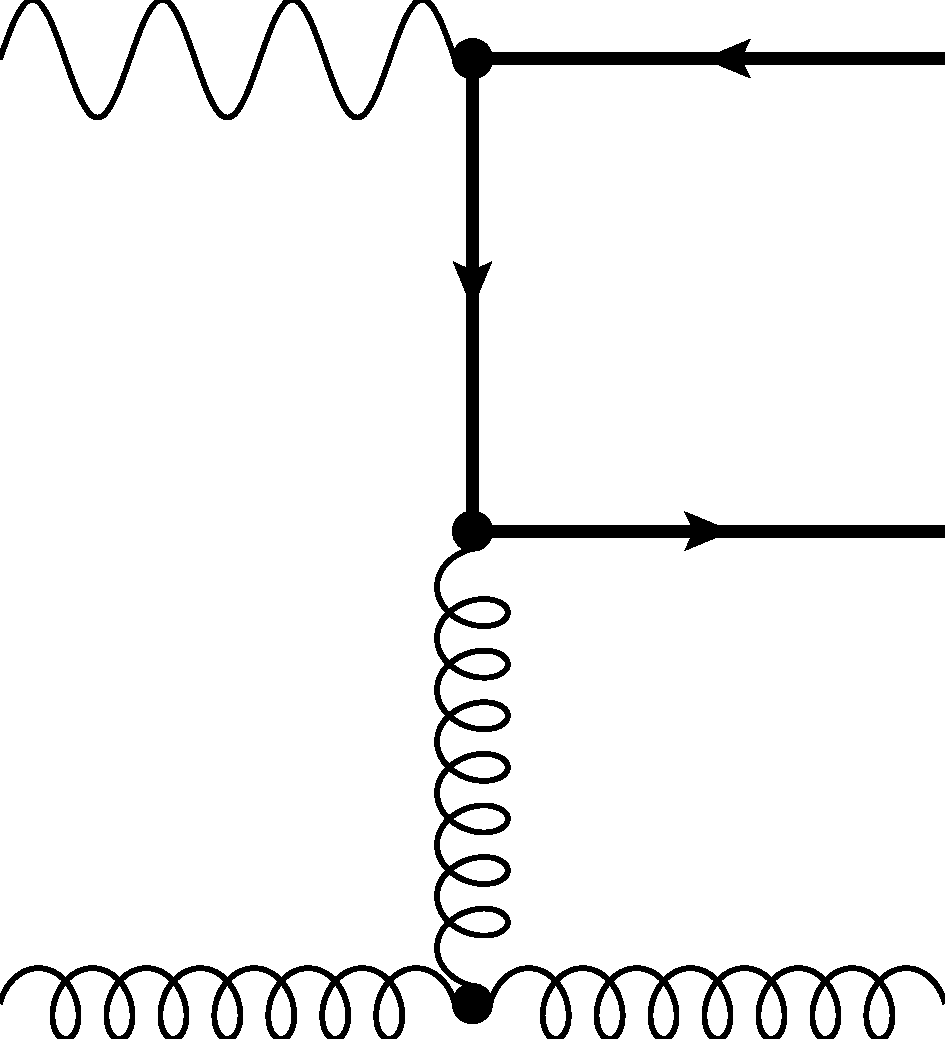
\includegraphics[width=\textwidth]{pyfeyn/nlo-g-4}
	\caption{\label{fig:FeynNLOg3g}}
\end{subfigure}
\caption{next-to-leading order Feynman diagrams for the single gluon radiation $i\varepsilon_{\Pgg}^\mu(q) \varepsilon_{\Pg}^\nu(k_1)\Md^{(1),g}_{j,\mu\nu}$. Four additional graphs are obtained by crossing the final heavy quark pair. With our choice of $\hat {\mathcal P}_{G/L}^{\Pg,\nu\nu'}$ the diagram \ref{fig:FeynNLOg3g} has to be regularized with the ghost contributions. }\label{fig:FeynNLOg}\fxerror{shift to appendix?}
\end{figure}

The result can than be written as
\begin{align}
M_k^{(1),\Pg} &= \hat {\mathcal P}_{k}^{\Pgg,\mu\mu'}\hat {\mathcal P}_{k}^{\Pg,\nu\nu'}\sum_{j,j'}{\Md^{(1),g}_{j,\mu\nu}\Md^{(1),g}_{j',\mu'\nu'}}^*\\
 &= 8g^4\mu_D^{-2\epsilon}e^2e_H^2 N_C C_F\left( C_A R_{k,OK} + 2C_F R_{k,QED}\right)
\end{align}
The partonic cross section is then given by:
\begin{align}
d\sigma_{k,\Pg}^{(1)} &= \frac{1}{2s'}\frac {K_{\Pgg\Pg}E_k(\epsilon)} 2 b_k(\epsilon) M_k^{(1),\Pg} dPS_{3}
\end{align}

For the gluonic part we shift the occuring soft ($x\rightarrow 1$) and collinear ($y\rightarrow -1$) poles from the matrix elements to the phase space by dividing by $t'\propto(1+y)(1-x)$ and $u'-q^2s_5/s\propto(1-x)$:
\begin{align}
dPS_{3,\Pg}' &= \frac{dPS_3}{t'(u'-q^2s_5/s)} = dPS_3 \cdot \left(\frac {2s}{{s'}^2}\right)^2\frac 1 {(1-x)^2(1-y)(1+y)}\\
 &= \frac {2T_\epsilon}{\pi} \left(\frac {{s'}^2} s\right)^{-1+\epsilon/2} (1-x)^{-1+\epsilon}(1-y^2)^{-1+\epsilon/2}dPS_2^{(5)}dy \sin^\epsilon(\theta_2)d\theta_2\\
{M_k^{(1),\Pg}}' &= t'(u'-q^2s_5/s)M_k^{(1),\Pg}\\
\Rightarrow d\sigma_{k,\Pg}^{(1)} &= \frac{1}{2s'}\frac {K_{\Pg\Pgg}E_k(\epsilon)} 2 b_k(\epsilon) {M_k^{(1),\Pg}}' dPS_{3,\Pg}'
\end{align}

The soft and collinear factors $(1-x)^{-1+\epsilon}$ and $(1-y^2)^{-1+\epsilon/2}$ can be replaced by generalized plus distributions\cite{Harris:1995tu}
\begin{align}
(1-x)^{-1+\epsilon} &\sim \left(\frac 1 {1-x}\right)_{\tilde\rho} + \epsilon \left(\frac{\ln(1-x)}{1-x}\right)_{\tilde \rho} + \delta(1-x)\left(\frac 1 \epsilon + 2\ln\tilde\beta + 2\epsilon\ln^2(\tilde\beta)\right) + O(\epsilon^2)\\
(1-y^2)^{-1+\epsilon} &\sim \frac 1 2\left(\left(\frac 1 {1+y}\right)_\omega + \left(\frac 1 {1-y}\right)_\omega\right) \nonumber\\
 &\hspace{20pt} + \left(\delta(1+y)+\delta(1-y)\right)\left(\frac 1 {2\epsilon} + \frac 1 2\ln(2\omega)\right) + O(\epsilon)\\
(1+y)^{-1+\epsilon} &\sim \left(\frac 1 {1+y}\right)_\omega + \delta(1+y)\left(\frac 1 \epsilon + \ln\omega\right) + O(\epsilon)
\end{align}
inside integration over smooth functions with $\tilde \beta = \sqrt{1-\tilde\rho}$. The distributions are defined by
\begin{align}
\int\limits_{\tilde\rho}^1\!\!dx\,f(x)\left(\frac 1 {1-x}\right)_{\tilde\rho} &= \int\limits_{\tilde\rho}^1\!\!dx\,\frac {f(x) - f(1)} {1-x}\\
\int\limits_{\tilde\rho}^1\!\!dx\,f(x)\left(\frac {\ln(1-x)} {1-x}\right)_{\tilde\rho} &= \int\limits_{\tilde\rho}^1\!\!dx\,\frac {f(x) - f(1)} {1-x}\ln(1-x)\\
\int\limits_{-1}^{-1+\omega}\!\!\!dy\,f(y)\left(\frac 1 {1+y}\right)_{\omega} &= \int\limits_{-1}^{-1+\omega}\!\!\!dy\,\frac {f(y)-f(-1)} {1+y}\\
\int\limits_{1-\omega}^{1}\!\!dy\,f(y)\left(\frac 1 {1-y}\right)_{\omega} &= \int\limits_{1-\omega}^{1}\!\!dy\,\frac {f(y)-f(1)} {1-y}
\end{align}
with $\rho^*\leq\tilde\rho < 1$ and $0<\omega\leq 2$. If the integration does not include a singularity the distribution sign can be dropped. From an analytical point of view the results may not depend on the specific choice of the regularisation parameters $\tilde\rho$ and $\omega$ but for any numerical purpose they may influence the rate of convergence or stability. For numerical computations we must also cut the poles out of the integrations
\begin{align}
\int\limits_{\rho^*}^1\!dx &\rightarrow \int\limits_{\rho^*}^{1-\delta_x}\!\!\!dx &\int\limits_{-1}^1\!dy &\rightarrow \int\limits_{-1+\delta_y}^{1}\!\!dy
\end{align}
If not stated otherwise we use as a default setup\fxerror{justify numbers?}:
\begin{align}
\tilde\rho &= \rho^* + \tilde x(1-\rho^*)\,\text{with}\, \tilde x=0.8 &\omega &= 1.0\\
\delta_x &= \num{1e-6} &\delta_y &=\num{7e-6}
\end{align}
\fxerror{shift (parts) to appendix?}

With the given distribution we can split the gluonic NLO part into three pieces\cite{Harris:1995tu}:
\begin{align}
d\sigma_{k,\Pg}^{(1)} &= d\sigma_{k,\Pg}^{(1),s} + d\sigma_{k,\Pg}^{(1),c-} + d\sigma_{k,\Pg}^{(1),f}
\end{align}
corresponding to the soft ($d\sigma_{k,\Pg}^{(1),s} \sim \delta(1-x)$), the collinear ($d\sigma_{k,\Pg}^{(1),c-} \sim \delta(1+y)$) and the finite parts ($d\sigma_{k,\Pg}^{(1),f} \sim \left(\frac 1 {1-x}\right)_{\tilde \rho}\left(\frac 1 {1+y}\right)_{\omega}$). Note that for $q^2 < 0$ there is only a single collinear contribution ($y\rightarrow -1$).

The soft matrix elements can be obtained from the above expressions by taking the soft limit $k_2\rightarrow 0$:
\begin{equation}
\lim_{k_2\rightarrow 0}\left(C_A R_{k,OK} + 2C_F R_{k,QED}\right) = \left(C_A S_{k,OK} + 2C_F S_{k,QED}\right) + O(1/s_4,1/s_3,1/t')
\end{equation}
with
\begin{align}
S_{k,OK}  &= 2\left(\frac{t_1}{t's_3} + \frac{u_1}{t's_4}-\frac{s-2m^2}{s_3s_4}\right)B_{k,QED}\\
S_{k,QED} &= 2\left(\frac{s-2m^2}{s_3s_4} - \frac{m^2}{s_3^2} - \frac{m^2}{s_4^2}\right)B_{k,QED}
\end{align}
Note that the einkonal factors multiplying the Born functions $B_{k,QED}$ neither depend on $q^2$ nor on the projection $k$. But the integrated expressions do depend on the regularization scheme, i.e. will here depend on $\tilde\rho$ rather then on a phasespace slicing parameter $\Delta$ as for inclusive calculations\cite{Laenen1993162}\fxerror{add my cite}. We find for the integrated expressions
\begin{align}
d\sigma_{k,\Pg}^{(1),s} &= \frac 1 {2s'}\frac {K_{\Pg\Pgg}E_k(\epsilon)} 2  b_k(\epsilon) M_k^{(1),S} dPS_2\\
M_k^{(1),S} &= 8g^4\mu_D^{-\epsilon}e^2e_H^2 N_C C_F C_\epsilon\left( C_A \tilde S_{OK} + 2C_F \tilde S_{QED}\right) B_{k,QED}
\end{align}
where the full expressions for $\tilde S$ can be found in \cite{Harris:1995tu} and the poles are given by
\begin{align}
\tilde S_{OK} &= 2\left(\frac 4 {\epsilon^2} + \left(\ln(-t_1/m^2) + \ln(-u_1/m^2) - \frac{2m^2-s}{s\beta}\ln(\chi) + 4\ln(\tilde\beta)\right)\frac 2 {\epsilon}\right) + O(\epsilon^0)\\
\tilde S_{QED} &=-2\cdot \left(1 - \frac{2m^2-s}{s\beta}\ln(\chi)\right)\frac 2 \epsilon + O(\epsilon^0)
\end{align}


\subsection{Light Quark Processes}
In next-to-leading order a new production mechanism enters, that is induced by a light quark, so we have to consider the process
\begin{equation}
\Pggx(q;\sigma_q) + \Pq(k_1;\sigma_{k_1}) \rightarrow \PQ(p_1)+\PaQ(p_2) + \Pq(k_2)
\end{equation}
All contributing diagrams are depicted in figure \fxerror{do} and the result can be written as
\begin{equation}
\hat\sum_{k,\sigma}\mathcal P_{k}^{\mu\mu'}\sum_{j,j'}{\Md^{(1),q}_{j,\mu}\Md^{(1),q}_{j',\mu'}}^* = 8g^4e^2 N_C C_F\left( e_H^2 A_{k,1} +  e_L^2 A_{k,2} +  e_L e_H A_{k,3} \right)
\end{equation}
where $e_L$ denotes the charge of the light quark $q$ in units of $e$.

The needed $2\rightarrow 3$ phase space has already been calculated in Section \ref{seq:NLO.g}



\section{Mass Factorization}
All collinear poles that arise in the NLO corrections to PGF subprocess $\sigma_{\vec\kappa,\Pg}^{(1)}$ or the Bethe-Heitler subprocess $\sigma_{\vec\kappa,\Pq}^{(1)}$ can be removed by a standard mass factorization 
\begin{align}
&{s'}^2\frac{d^2\sigma_{\vec \kappa,j}^{(1),fin}(s',t_1,u_1,\mu_F)}{dt_1du_1} = \lim_{\epsilon\rightarrow 0}\left[{s'}^2\frac{d^2\sigma_{\vec \kappa,j}^{(1)}(s',t_1,u_1,\epsilon)}{dt_1du_1} \right.\nonumber\\
 &\hspace{40pt}\left. -\int\limits_0^1\frac{dx_1}{x_1}\Gamma_{\kappa_2,\Pg j}^{(1)}(x_1,\mu_F^2,\mu_D,\epsilon)(x_1s')^2\frac{d^2\sigma_{\vec \kappa,\Pg}^{(0)}(x_1s',x_1t_1,u_1,\epsilon)}{d(x_1t_1)du_1} \right]
\end{align}
for $j=\{\Pg,\Pq\}$ and where $\Gamma_{\kappa_2,ij}^{(1)}$ is the first order correction to the transition functions $\Gamma_{\kappa_2,ij}$ for \textit{incoming} particle $j$ and \textit{outgoing} particle $i$ in projection $\kappa_2$:
\begin{align}
\Gamma_{\kappa_2,ij}^{(1)}(x,\mu_F^2,\mu_D,\epsilon) &= \frac{\alpha_s}{2\pi}\left(P_{\kappa_2,ij}^{(0)}(x)\frac{2}{\epsilon} + f_{\kappa_2,ij}^{(1)}(x,\mu_F^2,\mu_D^2)\right)
\end{align}
In the adopted $\MSbar$-scheme the $f_{\kappa_2,ij}^{(1)}$ take their usual form and we find
\begin{align}
\Gamma_{\kappa_2,ij}^{(1),\MSbar}(x,\mu_F^2,\mu_D,\epsilon) &= \frac{\alpha_s}{2\pi}P_{\kappa_2,ij}^{(0)}(x)\left(\frac{2}{\epsilon} +\gamma_E - \ln(4\pi) + \ln(\mu_F^2/m^2) - \ln(\mu_D^2/m^2)\right)\\
 &= 8\pi\alpha_s P_{\kappa_2,ij}^{(0)}(x) C_\epsilon \left(\frac{\mu_D^2}{m^2}\right)^{-\epsilon/2} \left(\frac{2}{\epsilon} + \ln(\mu_F^2/m^2)\right)
\end{align}
For the PGF subprocess we need the LO gluon-to-gluon splitting functions $P_{\kappa_2,\Pg\Pg}^{(0)}(x)$ given by\cite{Altarelli:1977zs}
\begin{align}
P_{\kappa_2,\Pg\Pg}^{(0)}(x) &= \Theta(1-\delta-x)P_{\kappa_2,\Pg\Pg}^{(0),H}(x)+\delta(1-x)\left(2C_A\ln(\delta)+\frac{\beta_0}{2}\right)
\end{align}
where we introduced another infrared cut-off $\delta$ to seperate soft collinear ($x\geq 1-\delta$) and hard collinear ($x<1-\delta$) gluons. By simple kinematics we find the relation $\delta=\Delta/(s'+t_1)$ that allows us to divide the collinear part again into a hard and a soft part, rendering each into a finite result. The functions $P_{\kappa_2,\Pg\Pg}^{(0),H}(x)$ have been already quoted in Eq. \ref{eq:PFggH} and \ref{eq:PgggH} and the needed splitting functions $P_{\kappa_2,\Pg\Pq}^{(0)}$ for the Bethe-Heitler subprocess have been given in Eqs. (\ref{eq:PGLgq}) and (\ref{eq:PPgq}), to denote the collinear poles there.

The final, finite partonic cross sections for the PGF subprocess is split, as discussed, into a hard contribution given by
\begin{align}
{s'}^2\frac{d^2\sigma_{\vec \kappa,\Pg}^{(1),H,fin}}{dt_1du_1} &=\alpha\alpha_Se_H^2K_{\Pg\Pgg}N_CC_F\left[-\frac 2 {u_1}P^H_{\kappa_2,\Pg\Pg}(x_1)\right. \nonumber\\
 &\hspace{40pt}\left\{ B^{(0)}_{\vec \kappa,\tQED}\left(\!\begin{array}{l}s'\rightarrow x_1s'\\t_1\rightarrow x_1 t_1\end{array}\!\!\right) \left(\ln\left(\frac{s_4^2}{m^2(s_4+m^2)}\right)-\ln(\mu_F^2/m^2)\right)\right. \nonumber\\
 &\hspace{40pt}\left.-2B^{(1)}_{\vec \kappa,\tQED}\left(\!\begin{array}{l}s'\rightarrow x_1s'\\t_1\rightarrow x_1 t_1\end{array}\!\!\right)\right\} \nonumber\\
 &\hspace{20pt}+C_A\frac{s_4}{2\pi(s_4+m^2)}\left(\int\!d\Omega_n\,R_{\vec \kappa,\tOK}\right)^{finite} \nonumber\\
 &\hspace{20pt}\left.+2C_F\frac{s_4}{2\pi(s_4+m^2)}\int\!d\Omega_4\,R_{\vec \kappa,\tQED}\right] \label{eq:Hfinal}
\end{align}
and the soft plus virtual contributions given by
\begin{align}
{s'}^2\frac{d^2\sigma_{\vec \kappa,\Pg}^{(1),S+V,fin}}{dt_1du_1} &=4\alpha\alpha_Se_H^2K_{\Pg\Pgg}N_CC_FB^{(0)}_{\vec \kappa,\tQED}\delta(s'+t_1+u_1)\left[C_A\ln^2(\Delta/m^2) \right.\nonumber\\
 &\hspace{20pt} + \ln(\Delta/m^2)\left(\left(\ln(-t_1/m^2)-\ln(-u_1/m^2)-\ln(\mu_F^2/m^2)\right)C_A \right. \nonumber\\
 &\hspace{80pt} \left. - \frac{2m^2-s}{s\beta}\ln(\chi)(C_A-2C_F) - 2C_F\right) \nonumber\\
 &\hspace{20pt}\left. + \frac {\beta_0^{lf}}{4}\left(\ln(\mu_R^2/m^2)- \ln(\mu_F^2/m^2)\right) +  f_{\vec \kappa}(s',u_1,t_1,q^2)\right] \label{eq:SVfinal}
\end{align}
where the functions $f_{\vec \kappa}$ in Eq. \ref{eq:SVfinal} contain logarithms and dilogarithms with different, complicated arguments, but they do not depend on $\Delta,\mu_F^2,\mu_R^2$ nor $n_f$ and $\beta_0^{lf} = (11C_A - 2n_{lf})/3$.

The corresponding finite, reduced partonic cross section for the light quark initiated processes reads
\begin{align}
{s'}^2\frac{d^2\sigma_{\vec \kappa,\Pq}^{(1),fin}}{dt_1du_1} &=\alpha\alpha_SK_{\Pq\Pgg}N_C\left[-\frac 1 {u_1}e_H^2P_{\kappa_2,\Pg\Pq}(x_1)\right. \nonumber\\
 &\hspace{40pt}\left\{B^{(0)}_{\vec \kappa,\tQED}\left(\!\begin{array}{l}s'\rightarrow x_1s'\\t_1\rightarrow x_1 t_1\end{array}\!\!\right) \left(\ln\left(\frac{s_4^2}{m^2(s_4+m^2)}\right)-\ln(\mu_F^2/m^2)-2\partial_\epsilon E_{\vec \kappa}(\epsilon=0)\right)\right. \nonumber\\
 &\hspace{40pt}\left.-2 B^{(1)}_{\vec \kappa,\tQED}\left(\!\begin{array}{l}s'\rightarrow x_1s'\\t_1\rightarrow x_1 t_1\end{array}\!\!\right)\right\} \nonumber\\
 &\hspace{20pt}+C_F\frac{s_4}{4\pi(s_4+m^2)}\left(\int\!d\Omega_n\,e_H^2A_{\vec \kappa,1}\right)^{finite} \nonumber\\
 &\hspace{20pt}\left.+C_F\frac{s_4}{4\pi(s_4+m^2)}\int\!d\Omega_4\,e_L^2A_{\vec \kappa,2} +C_F\frac{s_4}{4\pi(s_4+m^2)}\int\!d\Omega_4\,e_H e_L A_{\vec \kappa,3} \right] \label{eq:qfinal}\,.
\end{align}

Note that the hat contributions for $g_1(x,Q^2)$ to the NLO PGF and the Bethe-Heitler process as computed in \cite{Hekhorn:2018ywm} this way can be directly related to $B^{(1)}_{\tVV,2xg_1,\tQED}$, as in this calculation this variable is not longer vanishing. This way we have shown that the Larin-scheme and the HVBM-scheme are equivalent for this process up to NLO.


\section{Partonic Results}
The \textit{total} partonic cross sections can be computed by
\begin{align}
\sigma^{(n)}_{k,j}(s,q^2,m^2) &= \int\limits_{-s'(1+\beta)/2}^{-s'(1-\beta)/2} dt_1\int\limits_0^{s_{4,max}}ds_4 \frac{d^2\sigma^{(n),fin}_{k,j}(s',t_1,u_1,q^2)}{dt_1ds_4}\\
s_{4,max} &= \frac{s}{s' t_1}\left(t_1+\frac{s'(1-\beta)}{2}\right)\left(t_1+\frac{s'(1+\beta)}{2}\right)
\end{align}
where $k$ denotes as usual projection, $j\in\{\Pg,\Pq,\Paq\}$ is a parton index and we used $s_4 = s'+t_1+u_1$. The result can then be parametrised as
\begin{align}
&\sigma_{k,j}(s,q^2,m^2)\nonumber\\
 &= \sigma^{(0)}_{k,j}(s,q^2,m^2) + \sigma^{(1)}_{k,j}(s,q^2,m^2)\\
 &= \frac{\alpha\alpha_S}{m^2}\left(f_{k,j}^{(0)}(\eta,\xi) + 4\pi\left(f_{k,j}^{(1)}(\eta,\xi) + \ln(\mu_F^2/m^2)\bar f_{k,j}^{F,(1)}(\eta,\xi) + \ln(\mu_R^2/m^2)\bar f_{k,j}^{R,(1)}(\eta,\xi)\right)\right)
\end{align}
where each function $f_{k,j}$ depends on the scaling variables $\eta=1/\rho-1$ and $\xi=-q^2/m^2$ and can be further decomposed by the electric charges
\begin{align}
f_{k,\Pg}(\eta,\xi) &= e_H^2 c_{k,\Pg}(\eta,\xi)\\
f_{k,\Pq}(\eta,\xi) &= e_H^2 c_{k,\Pq}(\eta,\xi) + e_L^2 d_{k,\Pq}(\eta,\xi)
\end{align}
As already mentioned the interference term proportional to $e_H e_L$ vanishes for total cross sections.

\fxerror{how to arrange 3 equal images? shift to appendix?}
\fxerror{compare T and P?}

\pagebreak
\begin{figure}[ht!]
\centering
\begin{subfigure}[t]{\textwidth}
	% GNUPLOT: LaTeX picture with Postscript
\begingroup
  \makeatletter
  \providecommand\color[2][]{%
    \GenericError{(gnuplot) \space\space\space\@spaces}{%
      Package color not loaded in conjunction with
      terminal option `colourtext'%
    }{See the gnuplot documentation for explanation.%
    }{Either use 'blacktext' in gnuplot or load the package
      color.sty in LaTeX.}%
    \renewcommand\color[2][]{}%
  }%
  \providecommand\includegraphics[2][]{%
    \GenericError{(gnuplot) \space\space\space\@spaces}{%
      Package graphicx or graphics not loaded%
    }{See the gnuplot documentation for explanation.%
    }{The gnuplot epslatex terminal needs graphicx.sty or graphics.sty.}%
    \renewcommand\includegraphics[2][]{}%
  }%
  \providecommand\rotatebox[2]{#2}%
  \@ifundefined{ifGPcolor}{%
    \newif\ifGPcolor
    \GPcolorfalse
  }{}%
  \@ifundefined{ifGPblacktext}{%
    \newif\ifGPblacktext
    \GPblacktexttrue
  }{}%
  % define a \g@addto@macro without @ in the name:
  \let\gplgaddtomacro\g@addto@macro
  % define empty templates for all commands taking text:
  \gdef\gplbacktext{}%
  \gdef\gplfronttext{}%
  \makeatother
  \ifGPblacktext
    % no textcolor at all
    \def\colorrgb#1{}%
    \def\colorgray#1{}%
  \else
    % gray or color?
    \ifGPcolor
      \def\colorrgb#1{\color[rgb]{#1}}%
      \def\colorgray#1{\color[gray]{#1}}%
      \expandafter\def\csname LTw\endcsname{\color{white}}%
      \expandafter\def\csname LTb\endcsname{\color{black}}%
      \expandafter\def\csname LTa\endcsname{\color{black}}%
      \expandafter\def\csname LT0\endcsname{\color[rgb]{1,0,0}}%
      \expandafter\def\csname LT1\endcsname{\color[rgb]{0,1,0}}%
      \expandafter\def\csname LT2\endcsname{\color[rgb]{0,0,1}}%
      \expandafter\def\csname LT3\endcsname{\color[rgb]{1,0,1}}%
      \expandafter\def\csname LT4\endcsname{\color[rgb]{0,1,1}}%
      \expandafter\def\csname LT5\endcsname{\color[rgb]{1,1,0}}%
      \expandafter\def\csname LT6\endcsname{\color[rgb]{0,0,0}}%
      \expandafter\def\csname LT7\endcsname{\color[rgb]{1,0.3,0}}%
      \expandafter\def\csname LT8\endcsname{\color[rgb]{0.5,0.5,0.5}}%
    \else
      % gray
      \def\colorrgb#1{\color{black}}%
      \def\colorgray#1{\color[gray]{#1}}%
      \expandafter\def\csname LTw\endcsname{\color{white}}%
      \expandafter\def\csname LTb\endcsname{\color{black}}%
      \expandafter\def\csname LTa\endcsname{\color{black}}%
      \expandafter\def\csname LT0\endcsname{\color{black}}%
      \expandafter\def\csname LT1\endcsname{\color{black}}%
      \expandafter\def\csname LT2\endcsname{\color{black}}%
      \expandafter\def\csname LT3\endcsname{\color{black}}%
      \expandafter\def\csname LT4\endcsname{\color{black}}%
      \expandafter\def\csname LT5\endcsname{\color{black}}%
      \expandafter\def\csname LT6\endcsname{\color{black}}%
      \expandafter\def\csname LT7\endcsname{\color{black}}%
      \expandafter\def\csname LT8\endcsname{\color{black}}%
    \fi
  \fi
    \setlength{\unitlength}{0.0500bp}%
    \ifx\gptboxheight\undefined%
      \newlength{\gptboxheight}%
      \newlength{\gptboxwidth}%
      \newsavebox{\gptboxtext}%
    \fi%
    \setlength{\fboxrule}{0.5pt}%
    \setlength{\fboxsep}{1pt}%
\begin{picture}(7920.00,4082.40)%
    \gplgaddtomacro\gplbacktext{%
      \csname LTb\endcsname%
      \put(726,220){\makebox(0,0)[r]{\strut{} 0.0}}%
      \put(726,820){\makebox(0,0)[r]{\strut{} 0.2}}%
      \put(726,1419){\makebox(0,0)[r]{\strut{} 0.4}}%
      \put(726,2019){\makebox(0,0)[r]{\strut{} 0.6}}%
      \put(726,2619){\makebox(0,0)[r]{\strut{} 0.8}}%
      \put(726,3218){\makebox(0,0)[r]{\strut{} 1.0}}%
      \put(726,3818){\makebox(0,0)[r]{\strut{} 1.2}}%
      \put(858,0){\makebox(0,0){\strut{}$0.001$}}%
      \put(1969,0){\makebox(0,0){\strut{}$0.01$}}%
      \put(3079,0){\makebox(0,0){\strut{}$0.1$}}%
      \put(4190,0){\makebox(0,0){\strut{}$1$}}%
      \put(5301,0){\makebox(0,0){\strut{}$10$}}%
      \put(6411,0){\makebox(0,0){\strut{}$100$}}%
      \put(7522,0){\makebox(0,0){\strut{}$1000$}}%
      \put(991,3458){\makebox(0,0)[l]{\strut{}(a) $c_{T,g}^{(0)}(\eta)$}}%
    }%
    \gplgaddtomacro\gplfronttext{%
      \csname LTb\endcsname%
      \put(5611,3645){\makebox(0,0)[l]{\strut{}$Q^2=10^{-2}$}}%
      \csname LTb\endcsname%
      \put(5611,3425){\makebox(0,0)[l]{\strut{}$Q^2=10^0$}}%
      \csname LTb\endcsname%
      \put(5611,3205){\makebox(0,0)[l]{\strut{}$Q^2=10^1$}}%
      \csname LTb\endcsname%
      \put(5611,2985){\makebox(0,0)[l]{\strut{}$Q^2=10^2$}}%
      \csname LTb\endcsname%
      \put(5611,2765){\makebox(0,0)[l]{\strut{}$Q^2=10^3$}}%
    }%
    \gplbacktext
    \put(0,0){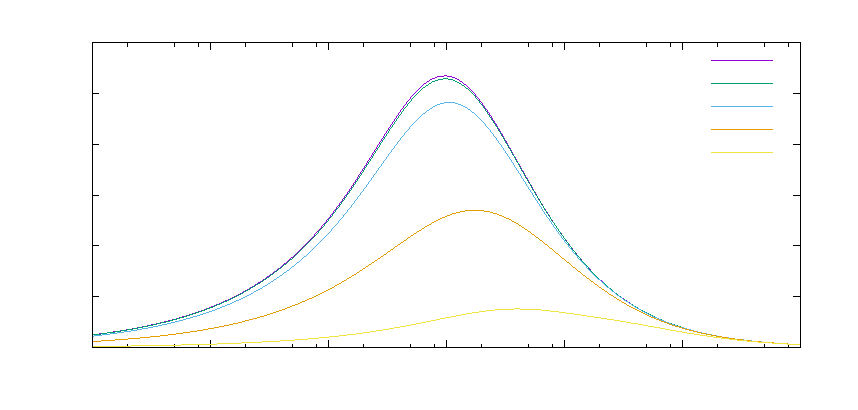
\includegraphics{img/cg0T}}%
    \gplfronttext
  \end{picture}%
\endgroup

	\caption{$c_{T,g}^{(0)}(\eta)$}
\end{subfigure}\\%
\begin{subfigure}[t]{\textwidth}
	% GNUPLOT: LaTeX picture with Postscript
\begingroup
  \makeatletter
  \providecommand\color[2][]{%
    \GenericError{(gnuplot) \space\space\space\@spaces}{%
      Package color not loaded in conjunction with
      terminal option `colourtext'%
    }{See the gnuplot documentation for explanation.%
    }{Either use 'blacktext' in gnuplot or load the package
      color.sty in LaTeX.}%
    \renewcommand\color[2][]{}%
  }%
  \providecommand\includegraphics[2][]{%
    \GenericError{(gnuplot) \space\space\space\@spaces}{%
      Package graphicx or graphics not loaded%
    }{See the gnuplot documentation for explanation.%
    }{The gnuplot epslatex terminal needs graphicx.sty or graphics.sty.}%
    \renewcommand\includegraphics[2][]{}%
  }%
  \providecommand\rotatebox[2]{#2}%
  \@ifundefined{ifGPcolor}{%
    \newif\ifGPcolor
    \GPcolorfalse
  }{}%
  \@ifundefined{ifGPblacktext}{%
    \newif\ifGPblacktext
    \GPblacktexttrue
  }{}%
  % define a \g@addto@macro without @ in the name:
  \let\gplgaddtomacro\g@addto@macro
  % define empty templates for all commands taking text:
  \gdef\gplbacktext{}%
  \gdef\gplfronttext{}%
  \makeatother
  \ifGPblacktext
    % no textcolor at all
    \def\colorrgb#1{}%
    \def\colorgray#1{}%
  \else
    % gray or color?
    \ifGPcolor
      \def\colorrgb#1{\color[rgb]{#1}}%
      \def\colorgray#1{\color[gray]{#1}}%
      \expandafter\def\csname LTw\endcsname{\color{white}}%
      \expandafter\def\csname LTb\endcsname{\color{black}}%
      \expandafter\def\csname LTa\endcsname{\color{black}}%
      \expandafter\def\csname LT0\endcsname{\color[rgb]{1,0,0}}%
      \expandafter\def\csname LT1\endcsname{\color[rgb]{0,1,0}}%
      \expandafter\def\csname LT2\endcsname{\color[rgb]{0,0,1}}%
      \expandafter\def\csname LT3\endcsname{\color[rgb]{1,0,1}}%
      \expandafter\def\csname LT4\endcsname{\color[rgb]{0,1,1}}%
      \expandafter\def\csname LT5\endcsname{\color[rgb]{1,1,0}}%
      \expandafter\def\csname LT6\endcsname{\color[rgb]{0,0,0}}%
      \expandafter\def\csname LT7\endcsname{\color[rgb]{1,0.3,0}}%
      \expandafter\def\csname LT8\endcsname{\color[rgb]{0.5,0.5,0.5}}%
    \else
      % gray
      \def\colorrgb#1{\color{black}}%
      \def\colorgray#1{\color[gray]{#1}}%
      \expandafter\def\csname LTw\endcsname{\color{white}}%
      \expandafter\def\csname LTb\endcsname{\color{black}}%
      \expandafter\def\csname LTa\endcsname{\color{black}}%
      \expandafter\def\csname LT0\endcsname{\color{black}}%
      \expandafter\def\csname LT1\endcsname{\color{black}}%
      \expandafter\def\csname LT2\endcsname{\color{black}}%
      \expandafter\def\csname LT3\endcsname{\color{black}}%
      \expandafter\def\csname LT4\endcsname{\color{black}}%
      \expandafter\def\csname LT5\endcsname{\color{black}}%
      \expandafter\def\csname LT6\endcsname{\color{black}}%
      \expandafter\def\csname LT7\endcsname{\color{black}}%
      \expandafter\def\csname LT8\endcsname{\color{black}}%
    \fi
  \fi
    \setlength{\unitlength}{0.0500bp}%
    \ifx\gptboxheight\undefined%
      \newlength{\gptboxheight}%
      \newlength{\gptboxwidth}%
      \newsavebox{\gptboxtext}%
    \fi%
    \setlength{\fboxrule}{0.5pt}%
    \setlength{\fboxsep}{1pt}%
\begin{picture}(7920.00,4082.40)%
    \gplgaddtomacro\gplbacktext{%
      \csname LTb\endcsname%
      \put(726,220){\makebox(0,0)[r]{\strut{}0.00}}%
      \put(726,734){\makebox(0,0)[r]{\strut{}0.02}}%
      \put(726,1248){\makebox(0,0)[r]{\strut{}0.04}}%
      \put(726,1762){\makebox(0,0)[r]{\strut{}0.06}}%
      \put(726,2276){\makebox(0,0)[r]{\strut{}0.08}}%
      \put(726,2790){\makebox(0,0)[r]{\strut{}0.10}}%
      \put(726,3304){\makebox(0,0)[r]{\strut{}0.12}}%
      \put(726,3818){\makebox(0,0)[r]{\strut{}0.14}}%
      \put(858,0){\makebox(0,0){\strut{}$0.001$}}%
      \put(1969,0){\makebox(0,0){\strut{}$0.01$}}%
      \put(3079,0){\makebox(0,0){\strut{}$0.1$}}%
      \put(4190,0){\makebox(0,0){\strut{}$1$}}%
      \put(5301,0){\makebox(0,0){\strut{}$10$}}%
      \put(6411,0){\makebox(0,0){\strut{}$100$}}%
      \put(7522,0){\makebox(0,0){\strut{}$1000$}}%
      \put(991,3458){\makebox(0,0)[l]{\strut{}(b) $c_{L,g}^{(0)}(\eta)$}}%
    }%
    \gplgaddtomacro\gplfronttext{%
      \csname LTb\endcsname%
      \put(5611,3645){\makebox(0,0)[l]{\strut{}$Q^2=10^{-2}$}}%
      \csname LTb\endcsname%
      \put(5611,3425){\makebox(0,0)[l]{\strut{}$Q^2=10^0$}}%
      \csname LTb\endcsname%
      \put(5611,3205){\makebox(0,0)[l]{\strut{}$Q^2=10^1$}}%
      \csname LTb\endcsname%
      \put(5611,2985){\makebox(0,0)[l]{\strut{}$Q^2=10^2$}}%
      \csname LTb\endcsname%
      \put(5611,2765){\makebox(0,0)[l]{\strut{}$Q^2=10^3$}}%
    }%
    \gplbacktext
    \put(0,0){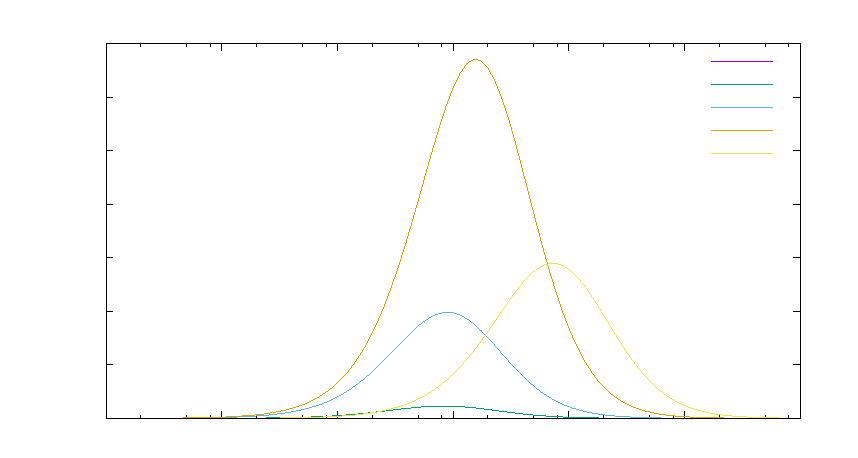
\includegraphics{img/cg0L}}%
    \gplfronttext
  \end{picture}%
\endgroup

	\caption{$c_{L,g}^{(0)}(\eta)$}
\end{subfigure}\\%
\begin{subfigure}[t]{\textwidth}
	% GNUPLOT: LaTeX picture with Postscript
\begingroup
  \makeatletter
  \providecommand\color[2][]{%
    \GenericError{(gnuplot) \space\space\space\@spaces}{%
      Package color not loaded in conjunction with
      terminal option `colourtext'%
    }{See the gnuplot documentation for explanation.%
    }{Either use 'blacktext' in gnuplot or load the package
      color.sty in LaTeX.}%
    \renewcommand\color[2][]{}%
  }%
  \providecommand\includegraphics[2][]{%
    \GenericError{(gnuplot) \space\space\space\@spaces}{%
      Package graphicx or graphics not loaded%
    }{See the gnuplot documentation for explanation.%
    }{The gnuplot epslatex terminal needs graphicx.sty or graphics.sty.}%
    \renewcommand\includegraphics[2][]{}%
  }%
  \providecommand\rotatebox[2]{#2}%
  \@ifundefined{ifGPcolor}{%
    \newif\ifGPcolor
    \GPcolorfalse
  }{}%
  \@ifundefined{ifGPblacktext}{%
    \newif\ifGPblacktext
    \GPblacktexttrue
  }{}%
  % define a \g@addto@macro without @ in the name:
  \let\gplgaddtomacro\g@addto@macro
  % define empty templates for all commands taking text:
  \gdef\gplbacktext{}%
  \gdef\gplfronttext{}%
  \makeatother
  \ifGPblacktext
    % no textcolor at all
    \def\colorrgb#1{}%
    \def\colorgray#1{}%
  \else
    % gray or color?
    \ifGPcolor
      \def\colorrgb#1{\color[rgb]{#1}}%
      \def\colorgray#1{\color[gray]{#1}}%
      \expandafter\def\csname LTw\endcsname{\color{white}}%
      \expandafter\def\csname LTb\endcsname{\color{black}}%
      \expandafter\def\csname LTa\endcsname{\color{black}}%
      \expandafter\def\csname LT0\endcsname{\color[rgb]{1,0,0}}%
      \expandafter\def\csname LT1\endcsname{\color[rgb]{0,1,0}}%
      \expandafter\def\csname LT2\endcsname{\color[rgb]{0,0,1}}%
      \expandafter\def\csname LT3\endcsname{\color[rgb]{1,0,1}}%
      \expandafter\def\csname LT4\endcsname{\color[rgb]{0,1,1}}%
      \expandafter\def\csname LT5\endcsname{\color[rgb]{1,1,0}}%
      \expandafter\def\csname LT6\endcsname{\color[rgb]{0,0,0}}%
      \expandafter\def\csname LT7\endcsname{\color[rgb]{1,0.3,0}}%
      \expandafter\def\csname LT8\endcsname{\color[rgb]{0.5,0.5,0.5}}%
    \else
      % gray
      \def\colorrgb#1{\color{black}}%
      \def\colorgray#1{\color[gray]{#1}}%
      \expandafter\def\csname LTw\endcsname{\color{white}}%
      \expandafter\def\csname LTb\endcsname{\color{black}}%
      \expandafter\def\csname LTa\endcsname{\color{black}}%
      \expandafter\def\csname LT0\endcsname{\color{black}}%
      \expandafter\def\csname LT1\endcsname{\color{black}}%
      \expandafter\def\csname LT2\endcsname{\color{black}}%
      \expandafter\def\csname LT3\endcsname{\color{black}}%
      \expandafter\def\csname LT4\endcsname{\color{black}}%
      \expandafter\def\csname LT5\endcsname{\color{black}}%
      \expandafter\def\csname LT6\endcsname{\color{black}}%
      \expandafter\def\csname LT7\endcsname{\color{black}}%
      \expandafter\def\csname LT8\endcsname{\color{black}}%
    \fi
  \fi
    \setlength{\unitlength}{0.0500bp}%
    \ifx\gptboxheight\undefined%
      \newlength{\gptboxheight}%
      \newlength{\gptboxwidth}%
      \newsavebox{\gptboxtext}%
    \fi%
    \setlength{\fboxrule}{0.5pt}%
    \setlength{\fboxsep}{1pt}%
\begin{picture}(7920.00,4082.40)%
    \gplgaddtomacro\gplbacktext{%
      \csname LTb\endcsname%
      \put(726,220){\makebox(0,0)[r]{\strut{}-0.2}}%
      \put(726,734){\makebox(0,0)[r]{\strut{}-0.1}}%
      \put(726,1248){\makebox(0,0)[r]{\strut{}0.0}}%
      \put(726,1762){\makebox(0,0)[r]{\strut{}0.1}}%
      \put(726,2276){\makebox(0,0)[r]{\strut{}0.2}}%
      \put(726,2790){\makebox(0,0)[r]{\strut{}0.3}}%
      \put(726,3304){\makebox(0,0)[r]{\strut{}0.4}}%
      \put(726,3818){\makebox(0,0)[r]{\strut{}0.5}}%
      \put(858,0){\makebox(0,0){\strut{}$0.001$}}%
      \put(1969,0){\makebox(0,0){\strut{}$0.01$}}%
      \put(3079,0){\makebox(0,0){\strut{}$0.1$}}%
      \put(4190,0){\makebox(0,0){\strut{}$1$}}%
      \put(5301,0){\makebox(0,0){\strut{}$10$}}%
      \put(6411,0){\makebox(0,0){\strut{}$100$}}%
      \put(7522,0){\makebox(0,0){\strut{}$1000$}}%
      \put(991,3458){\makebox(0,0)[l]{\strut{}(c) $c_{P,g}^{(0)}(\eta)$}}%
    }%
    \gplgaddtomacro\gplfronttext{%
      \csname LTb\endcsname%
      \put(5611,3645){\makebox(0,0)[l]{\strut{}$Q^2=10^{-2}$}}%
      \csname LTb\endcsname%
      \put(5611,3425){\makebox(0,0)[l]{\strut{}$Q^2=10^0$}}%
      \csname LTb\endcsname%
      \put(5611,3205){\makebox(0,0)[l]{\strut{}$Q^2=10^1$}}%
      \csname LTb\endcsname%
      \put(5611,2985){\makebox(0,0)[l]{\strut{}$Q^2=10^2$}}%
      \csname LTb\endcsname%
      \put(5611,2765){\makebox(0,0)[l]{\strut{}$Q^2=10^3$}}%
    }%
    \gplbacktext
    \put(0,0){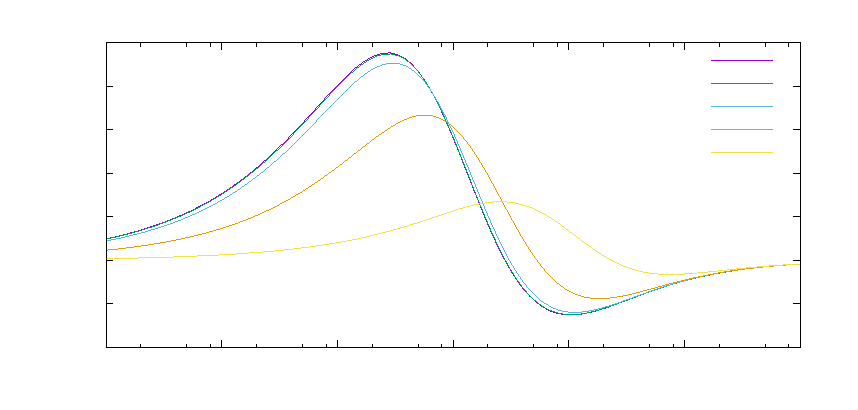
\includegraphics{img/cg0P}}%
    \gplfronttext
  \end{picture}%
\endgroup

	\caption{$c_{P,g}^{(0)}(\eta)$}
\end{subfigure}
\caption{leading order scaling functions $c_{k,g}^{(0)}(\eta,\xi)$ plotted as function of $\eta=s/(4m^2)-1$ for different values of $Q^2$ in units of $\si{\GeV^2}$ at $m=\SI{4.75}{\GeV}$ (i.e. different values of $\xi=Q^2/m^2$) }\label{fig:cg0}
\end{figure}

\pagebreak
\begin{figure}[ht!]
\centering
\begin{subfigure}[t]{\textwidth}
	% GNUPLOT: LaTeX picture with Postscript
\begingroup
  \makeatletter
  \providecommand\color[2][]{%
    \GenericError{(gnuplot) \space\space\space\@spaces}{%
      Package color not loaded in conjunction with
      terminal option `colourtext'%
    }{See the gnuplot documentation for explanation.%
    }{Either use 'blacktext' in gnuplot or load the package
      color.sty in LaTeX.}%
    \renewcommand\color[2][]{}%
  }%
  \providecommand\includegraphics[2][]{%
    \GenericError{(gnuplot) \space\space\space\@spaces}{%
      Package graphicx or graphics not loaded%
    }{See the gnuplot documentation for explanation.%
    }{The gnuplot epslatex terminal needs graphicx.sty or graphics.sty.}%
    \renewcommand\includegraphics[2][]{}%
  }%
  \providecommand\rotatebox[2]{#2}%
  \@ifundefined{ifGPcolor}{%
    \newif\ifGPcolor
    \GPcolorfalse
  }{}%
  \@ifundefined{ifGPblacktext}{%
    \newif\ifGPblacktext
    \GPblacktexttrue
  }{}%
  % define a \g@addto@macro without @ in the name:
  \let\gplgaddtomacro\g@addto@macro
  % define empty templates for all commands taking text:
  \gdef\gplbacktext{}%
  \gdef\gplfronttext{}%
  \makeatother
  \ifGPblacktext
    % no textcolor at all
    \def\colorrgb#1{}%
    \def\colorgray#1{}%
  \else
    % gray or color?
    \ifGPcolor
      \def\colorrgb#1{\color[rgb]{#1}}%
      \def\colorgray#1{\color[gray]{#1}}%
      \expandafter\def\csname LTw\endcsname{\color{white}}%
      \expandafter\def\csname LTb\endcsname{\color{black}}%
      \expandafter\def\csname LTa\endcsname{\color{black}}%
      \expandafter\def\csname LT0\endcsname{\color[rgb]{1,0,0}}%
      \expandafter\def\csname LT1\endcsname{\color[rgb]{0,1,0}}%
      \expandafter\def\csname LT2\endcsname{\color[rgb]{0,0,1}}%
      \expandafter\def\csname LT3\endcsname{\color[rgb]{1,0,1}}%
      \expandafter\def\csname LT4\endcsname{\color[rgb]{0,1,1}}%
      \expandafter\def\csname LT5\endcsname{\color[rgb]{1,1,0}}%
      \expandafter\def\csname LT6\endcsname{\color[rgb]{0,0,0}}%
      \expandafter\def\csname LT7\endcsname{\color[rgb]{1,0.3,0}}%
      \expandafter\def\csname LT8\endcsname{\color[rgb]{0.5,0.5,0.5}}%
    \else
      % gray
      \def\colorrgb#1{\color{black}}%
      \def\colorgray#1{\color[gray]{#1}}%
      \expandafter\def\csname LTw\endcsname{\color{white}}%
      \expandafter\def\csname LTb\endcsname{\color{black}}%
      \expandafter\def\csname LTa\endcsname{\color{black}}%
      \expandafter\def\csname LT0\endcsname{\color{black}}%
      \expandafter\def\csname LT1\endcsname{\color{black}}%
      \expandafter\def\csname LT2\endcsname{\color{black}}%
      \expandafter\def\csname LT3\endcsname{\color{black}}%
      \expandafter\def\csname LT4\endcsname{\color{black}}%
      \expandafter\def\csname LT5\endcsname{\color{black}}%
      \expandafter\def\csname LT6\endcsname{\color{black}}%
      \expandafter\def\csname LT7\endcsname{\color{black}}%
      \expandafter\def\csname LT8\endcsname{\color{black}}%
    \fi
  \fi
    \setlength{\unitlength}{0.0500bp}%
    \ifx\gptboxheight\undefined%
      \newlength{\gptboxheight}%
      \newlength{\gptboxwidth}%
      \newsavebox{\gptboxtext}%
    \fi%
    \setlength{\fboxrule}{0.5pt}%
    \setlength{\fboxsep}{1pt}%
\begin{picture}(7920.00,3628.80)%
    \gplgaddtomacro\gplbacktext{%
      \csname LTb\endcsname%
      \put(726,440){\makebox(0,0)[r]{\strut{}-0.1}}%
      \put(726,806){\makebox(0,0)[r]{\strut{}0.0}}%
      \put(726,1171){\makebox(0,0)[r]{\strut{}0.1}}%
      \put(726,1537){\makebox(0,0)[r]{\strut{}0.1}}%
      \put(726,1902){\makebox(0,0)[r]{\strut{}0.2}}%
      \put(726,2268){\makebox(0,0)[r]{\strut{}0.2}}%
      \put(726,2633){\makebox(0,0)[r]{\strut{}0.2}}%
      \put(726,2999){\makebox(0,0)[r]{\strut{}0.3}}%
      \put(726,3364){\makebox(0,0)[r]{\strut{}0.3}}%
      \put(858,220){\makebox(0,0){\strut{}$0.001$}}%
      \put(1969,220){\makebox(0,0){\strut{}$0.01$}}%
      \put(3079,220){\makebox(0,0){\strut{}$0.1$}}%
      \put(4190,220){\makebox(0,0){\strut{}$1$}}%
      \put(5301,220){\makebox(0,0){\strut{}$10$}}%
      \put(6411,220){\makebox(0,0){\strut{}$100$}}%
      \put(7522,220){\makebox(0,0){\strut{}$1000$}}%
    }%
    \gplgaddtomacro\gplfronttext{%
      \csname LTb\endcsname%
      \put(4077,3108){\makebox(0,0)[l]{\strut{}$Q^2=10^{-2}$}}%
      \csname LTb\endcsname%
      \put(4077,2888){\makebox(0,0)[l]{\strut{}$Q^2=10^0$}}%
      \csname LTb\endcsname%
      \put(4077,2668){\makebox(0,0)[l]{\strut{}$Q^2=10^1$}}%
      \csname LTb\endcsname%
      \put(4077,2448){\makebox(0,0)[l]{\strut{}$Q^2=10^2$}}%
      \csname LTb\endcsname%
      \put(4077,2228){\makebox(0,0)[l]{\strut{}$Q^2=10^3$}}%
    }%
    \gplbacktext
    \put(0,0){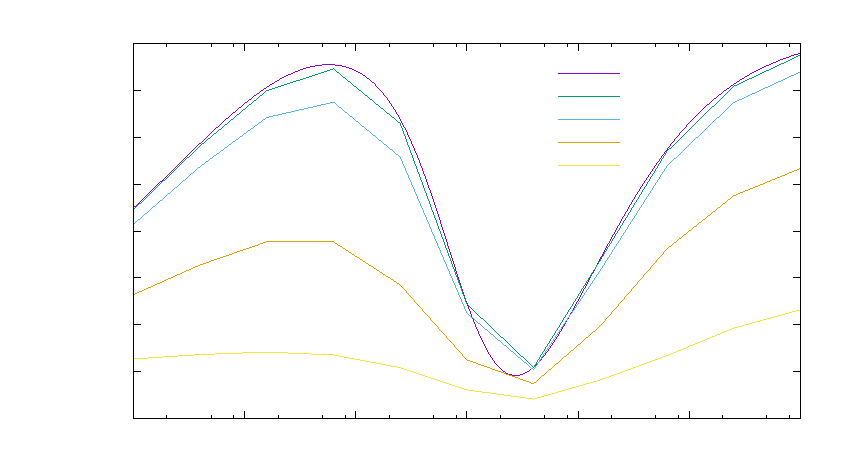
\includegraphics{img/cg1T}}%
    \gplfronttext
  \end{picture}%
\endgroup

	\caption{$c_{T,g}^{(1)}(\eta)$}
\end{subfigure}\\%
\begin{subfigure}[t]{\textwidth}
	% GNUPLOT: LaTeX picture with Postscript
\begingroup
  \makeatletter
  \providecommand\color[2][]{%
    \GenericError{(gnuplot) \space\space\space\@spaces}{%
      Package color not loaded in conjunction with
      terminal option `colourtext'%
    }{See the gnuplot documentation for explanation.%
    }{Either use 'blacktext' in gnuplot or load the package
      color.sty in LaTeX.}%
    \renewcommand\color[2][]{}%
  }%
  \providecommand\includegraphics[2][]{%
    \GenericError{(gnuplot) \space\space\space\@spaces}{%
      Package graphicx or graphics not loaded%
    }{See the gnuplot documentation for explanation.%
    }{The gnuplot epslatex terminal needs graphicx.sty or graphics.sty.}%
    \renewcommand\includegraphics[2][]{}%
  }%
  \providecommand\rotatebox[2]{#2}%
  \@ifundefined{ifGPcolor}{%
    \newif\ifGPcolor
    \GPcolorfalse
  }{}%
  \@ifundefined{ifGPblacktext}{%
    \newif\ifGPblacktext
    \GPblacktexttrue
  }{}%
  % define a \g@addto@macro without @ in the name:
  \let\gplgaddtomacro\g@addto@macro
  % define empty templates for all commands taking text:
  \gdef\gplbacktext{}%
  \gdef\gplfronttext{}%
  \makeatother
  \ifGPblacktext
    % no textcolor at all
    \def\colorrgb#1{}%
    \def\colorgray#1{}%
  \else
    % gray or color?
    \ifGPcolor
      \def\colorrgb#1{\color[rgb]{#1}}%
      \def\colorgray#1{\color[gray]{#1}}%
      \expandafter\def\csname LTw\endcsname{\color{white}}%
      \expandafter\def\csname LTb\endcsname{\color{black}}%
      \expandafter\def\csname LTa\endcsname{\color{black}}%
      \expandafter\def\csname LT0\endcsname{\color[rgb]{1,0,0}}%
      \expandafter\def\csname LT1\endcsname{\color[rgb]{0,1,0}}%
      \expandafter\def\csname LT2\endcsname{\color[rgb]{0,0,1}}%
      \expandafter\def\csname LT3\endcsname{\color[rgb]{1,0,1}}%
      \expandafter\def\csname LT4\endcsname{\color[rgb]{0,1,1}}%
      \expandafter\def\csname LT5\endcsname{\color[rgb]{1,1,0}}%
      \expandafter\def\csname LT6\endcsname{\color[rgb]{0,0,0}}%
      \expandafter\def\csname LT7\endcsname{\color[rgb]{1,0.3,0}}%
      \expandafter\def\csname LT8\endcsname{\color[rgb]{0.5,0.5,0.5}}%
    \else
      % gray
      \def\colorrgb#1{\color{black}}%
      \def\colorgray#1{\color[gray]{#1}}%
      \expandafter\def\csname LTw\endcsname{\color{white}}%
      \expandafter\def\csname LTb\endcsname{\color{black}}%
      \expandafter\def\csname LTa\endcsname{\color{black}}%
      \expandafter\def\csname LT0\endcsname{\color{black}}%
      \expandafter\def\csname LT1\endcsname{\color{black}}%
      \expandafter\def\csname LT2\endcsname{\color{black}}%
      \expandafter\def\csname LT3\endcsname{\color{black}}%
      \expandafter\def\csname LT4\endcsname{\color{black}}%
      \expandafter\def\csname LT5\endcsname{\color{black}}%
      \expandafter\def\csname LT6\endcsname{\color{black}}%
      \expandafter\def\csname LT7\endcsname{\color{black}}%
      \expandafter\def\csname LT8\endcsname{\color{black}}%
    \fi
  \fi
    \setlength{\unitlength}{0.0500bp}%
    \ifx\gptboxheight\undefined%
      \newlength{\gptboxheight}%
      \newlength{\gptboxwidth}%
      \newsavebox{\gptboxtext}%
    \fi%
    \setlength{\fboxrule}{0.5pt}%
    \setlength{\fboxsep}{1pt}%
\begin{picture}(7920.00,4082.40)%
    \gplgaddtomacro\gplbacktext{%
      \csname LTb\endcsname%
      \put(990,220){\makebox(0,0)[r]{\strut{}-0.015}}%
      \put(990,620){\makebox(0,0)[r]{\strut{}-0.010}}%
      \put(990,1020){\makebox(0,0)[r]{\strut{}-0.005}}%
      \put(990,1419){\makebox(0,0)[r]{\strut{}0.000}}%
      \put(990,1819){\makebox(0,0)[r]{\strut{}0.005}}%
      \put(990,2219){\makebox(0,0)[r]{\strut{}0.010}}%
      \put(990,2619){\makebox(0,0)[r]{\strut{}0.015}}%
      \put(990,3018){\makebox(0,0)[r]{\strut{}0.020}}%
      \put(990,3418){\makebox(0,0)[r]{\strut{}0.025}}%
      \put(990,3818){\makebox(0,0)[r]{\strut{}0.030}}%
      \put(1122,0){\makebox(0,0){\strut{}$0.001$}}%
      \put(2189,0){\makebox(0,0){\strut{}$0.01$}}%
      \put(3255,0){\makebox(0,0){\strut{}$0.1$}}%
      \put(4322,0){\makebox(0,0){\strut{}$1$}}%
      \put(5389,0){\makebox(0,0){\strut{}$10$}}%
      \put(6455,0){\makebox(0,0){\strut{}$100$}}%
      \put(7522,0){\makebox(0,0){\strut{}$1000$}}%
      \put(1250,472){\makebox(0,0)[l]{\strut{}(b) $c_{L,g}^{(1)}(\eta)$}}%
    }%
    \gplgaddtomacro\gplfronttext{%
      \csname LTb\endcsname%
      \put(1254,3645){\makebox(0,0)[l]{\strut{}$Q^2=10^{-2}$}}%
      \csname LTb\endcsname%
      \put(1254,3425){\makebox(0,0)[l]{\strut{}$Q^2=10^0$}}%
      \csname LTb\endcsname%
      \put(1254,3205){\makebox(0,0)[l]{\strut{}$Q^2=10^1$}}%
      \csname LTb\endcsname%
      \put(1254,2985){\makebox(0,0)[l]{\strut{}$Q^2=10^2$}}%
      \csname LTb\endcsname%
      \put(1254,2765){\makebox(0,0)[l]{\strut{}$Q^2=10^3$}}%
    }%
    \gplbacktext
    \put(0,0){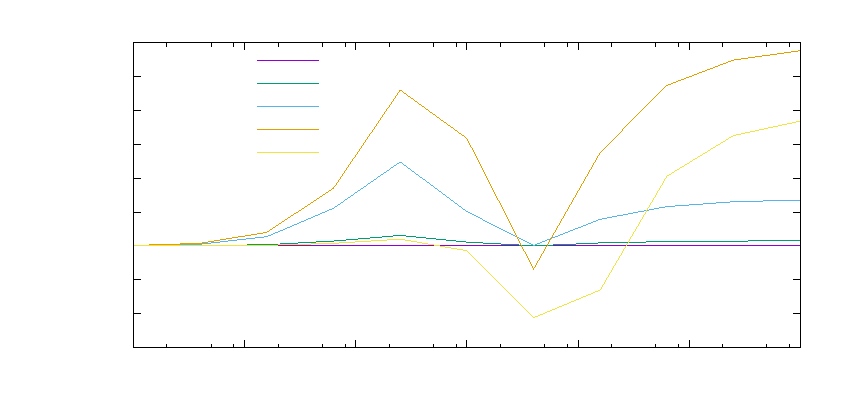
\includegraphics{img/cg1L}}%
    \gplfronttext
  \end{picture}%
\endgroup

	\caption{$c_{L,g}^{(1)}(\eta)$}
\end{subfigure}\\%
\begin{subfigure}[t]{\textwidth}
	% GNUPLOT: LaTeX picture with Postscript
\begingroup
  \makeatletter
  \providecommand\color[2][]{%
    \GenericError{(gnuplot) \space\space\space\@spaces}{%
      Package color not loaded in conjunction with
      terminal option `colourtext'%
    }{See the gnuplot documentation for explanation.%
    }{Either use 'blacktext' in gnuplot or load the package
      color.sty in LaTeX.}%
    \renewcommand\color[2][]{}%
  }%
  \providecommand\includegraphics[2][]{%
    \GenericError{(gnuplot) \space\space\space\@spaces}{%
      Package graphicx or graphics not loaded%
    }{See the gnuplot documentation for explanation.%
    }{The gnuplot epslatex terminal needs graphicx.sty or graphics.sty.}%
    \renewcommand\includegraphics[2][]{}%
  }%
  \providecommand\rotatebox[2]{#2}%
  \@ifundefined{ifGPcolor}{%
    \newif\ifGPcolor
    \GPcolorfalse
  }{}%
  \@ifundefined{ifGPblacktext}{%
    \newif\ifGPblacktext
    \GPblacktexttrue
  }{}%
  % define a \g@addto@macro without @ in the name:
  \let\gplgaddtomacro\g@addto@macro
  % define empty templates for all commands taking text:
  \gdef\gplbacktext{}%
  \gdef\gplfronttext{}%
  \makeatother
  \ifGPblacktext
    % no textcolor at all
    \def\colorrgb#1{}%
    \def\colorgray#1{}%
  \else
    % gray or color?
    \ifGPcolor
      \def\colorrgb#1{\color[rgb]{#1}}%
      \def\colorgray#1{\color[gray]{#1}}%
      \expandafter\def\csname LTw\endcsname{\color{white}}%
      \expandafter\def\csname LTb\endcsname{\color{black}}%
      \expandafter\def\csname LTa\endcsname{\color{black}}%
      \expandafter\def\csname LT0\endcsname{\color[rgb]{1,0,0}}%
      \expandafter\def\csname LT1\endcsname{\color[rgb]{0,1,0}}%
      \expandafter\def\csname LT2\endcsname{\color[rgb]{0,0,1}}%
      \expandafter\def\csname LT3\endcsname{\color[rgb]{1,0,1}}%
      \expandafter\def\csname LT4\endcsname{\color[rgb]{0,1,1}}%
      \expandafter\def\csname LT5\endcsname{\color[rgb]{1,1,0}}%
      \expandafter\def\csname LT6\endcsname{\color[rgb]{0,0,0}}%
      \expandafter\def\csname LT7\endcsname{\color[rgb]{1,0.3,0}}%
      \expandafter\def\csname LT8\endcsname{\color[rgb]{0.5,0.5,0.5}}%
    \else
      % gray
      \def\colorrgb#1{\color{black}}%
      \def\colorgray#1{\color[gray]{#1}}%
      \expandafter\def\csname LTw\endcsname{\color{white}}%
      \expandafter\def\csname LTb\endcsname{\color{black}}%
      \expandafter\def\csname LTa\endcsname{\color{black}}%
      \expandafter\def\csname LT0\endcsname{\color{black}}%
      \expandafter\def\csname LT1\endcsname{\color{black}}%
      \expandafter\def\csname LT2\endcsname{\color{black}}%
      \expandafter\def\csname LT3\endcsname{\color{black}}%
      \expandafter\def\csname LT4\endcsname{\color{black}}%
      \expandafter\def\csname LT5\endcsname{\color{black}}%
      \expandafter\def\csname LT6\endcsname{\color{black}}%
      \expandafter\def\csname LT7\endcsname{\color{black}}%
      \expandafter\def\csname LT8\endcsname{\color{black}}%
    \fi
  \fi
    \setlength{\unitlength}{0.0500bp}%
    \ifx\gptboxheight\undefined%
      \newlength{\gptboxheight}%
      \newlength{\gptboxwidth}%
      \newsavebox{\gptboxtext}%
    \fi%
    \setlength{\fboxrule}{0.5pt}%
    \setlength{\fboxsep}{1pt}%
\begin{picture}(7920.00,3628.80)%
    \gplgaddtomacro\gplbacktext{%
      \csname LTb\endcsname%
      \put(726,440){\makebox(0,0)[r]{\strut{}-0.2}}%
      \put(726,765){\makebox(0,0)[r]{\strut{}-0.1}}%
      \put(726,1090){\makebox(0,0)[r]{\strut{}-0.1}}%
      \put(726,1415){\makebox(0,0)[r]{\strut{}0.0}}%
      \put(726,1740){\makebox(0,0)[r]{\strut{}0.0}}%
      \put(726,2064){\makebox(0,0)[r]{\strut{}0.1}}%
      \put(726,2389){\makebox(0,0)[r]{\strut{}0.1}}%
      \put(726,2714){\makebox(0,0)[r]{\strut{}0.2}}%
      \put(726,3039){\makebox(0,0)[r]{\strut{}0.2}}%
      \put(726,3364){\makebox(0,0)[r]{\strut{}0.3}}%
      \put(858,220){\makebox(0,0){\strut{}$0.001$}}%
      \put(1969,220){\makebox(0,0){\strut{}$0.01$}}%
      \put(3079,220){\makebox(0,0){\strut{}$0.1$}}%
      \put(4190,220){\makebox(0,0){\strut{}$1$}}%
      \put(5301,220){\makebox(0,0){\strut{}$10$}}%
      \put(6411,220){\makebox(0,0){\strut{}$100$}}%
      \put(7522,220){\makebox(0,0){\strut{}$1000$}}%
    }%
    \gplgaddtomacro\gplfronttext{%
      \csname LTb\endcsname%
      \put(5611,3191){\makebox(0,0)[l]{\strut{}$Q^2=10^{-2}$}}%
      \csname LTb\endcsname%
      \put(5611,2971){\makebox(0,0)[l]{\strut{}$Q^2=10^0$}}%
      \csname LTb\endcsname%
      \put(5611,2751){\makebox(0,0)[l]{\strut{}$Q^2=10^1$}}%
      \csname LTb\endcsname%
      \put(5611,2531){\makebox(0,0)[l]{\strut{}$Q^2=10^2$}}%
      \csname LTb\endcsname%
      \put(5611,2311){\makebox(0,0)[l]{\strut{}$Q^2=10^3$}}%
    }%
    \gplbacktext
    \put(0,0){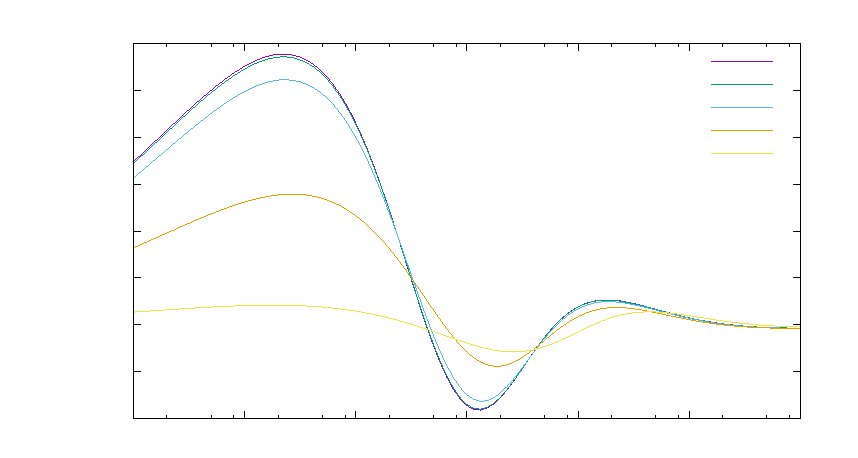
\includegraphics{img/cg1P}}%
    \gplfronttext
  \end{picture}%
\endgroup

	\caption{$c_{P,g}^{(1)}(\eta)$}
\end{subfigure}
\caption{next-to-leading order scaling functions $c_{k,g}^{(1)}(\eta,\xi)$ plotted as function of $\eta=s/(4m^2)-1$ for different values of $Q^2$ in units of $\si{\GeV^2}$ at $m=\SI{4.75}{\GeV}$ (i.e. different values of $\xi=Q^2/m^2$) }\label{fig:cg1}
\end{figure}

\pagebreak
\begin{figure}[ht!]
\centering
\begin{subfigure}[t]{\textwidth}
	% GNUPLOT: LaTeX picture with Postscript
\begingroup
  \makeatletter
  \providecommand\color[2][]{%
    \GenericError{(gnuplot) \space\space\space\@spaces}{%
      Package color not loaded in conjunction with
      terminal option `colourtext'%
    }{See the gnuplot documentation for explanation.%
    }{Either use 'blacktext' in gnuplot or load the package
      color.sty in LaTeX.}%
    \renewcommand\color[2][]{}%
  }%
  \providecommand\includegraphics[2][]{%
    \GenericError{(gnuplot) \space\space\space\@spaces}{%
      Package graphicx or graphics not loaded%
    }{See the gnuplot documentation for explanation.%
    }{The gnuplot epslatex terminal needs graphicx.sty or graphics.sty.}%
    \renewcommand\includegraphics[2][]{}%
  }%
  \providecommand\rotatebox[2]{#2}%
  \@ifundefined{ifGPcolor}{%
    \newif\ifGPcolor
    \GPcolorfalse
  }{}%
  \@ifundefined{ifGPblacktext}{%
    \newif\ifGPblacktext
    \GPblacktexttrue
  }{}%
  % define a \g@addto@macro without @ in the name:
  \let\gplgaddtomacro\g@addto@macro
  % define empty templates for all commands taking text:
  \gdef\gplbacktext{}%
  \gdef\gplfronttext{}%
  \makeatother
  \ifGPblacktext
    % no textcolor at all
    \def\colorrgb#1{}%
    \def\colorgray#1{}%
  \else
    % gray or color?
    \ifGPcolor
      \def\colorrgb#1{\color[rgb]{#1}}%
      \def\colorgray#1{\color[gray]{#1}}%
      \expandafter\def\csname LTw\endcsname{\color{white}}%
      \expandafter\def\csname LTb\endcsname{\color{black}}%
      \expandafter\def\csname LTa\endcsname{\color{black}}%
      \expandafter\def\csname LT0\endcsname{\color[rgb]{1,0,0}}%
      \expandafter\def\csname LT1\endcsname{\color[rgb]{0,1,0}}%
      \expandafter\def\csname LT2\endcsname{\color[rgb]{0,0,1}}%
      \expandafter\def\csname LT3\endcsname{\color[rgb]{1,0,1}}%
      \expandafter\def\csname LT4\endcsname{\color[rgb]{0,1,1}}%
      \expandafter\def\csname LT5\endcsname{\color[rgb]{1,1,0}}%
      \expandafter\def\csname LT6\endcsname{\color[rgb]{0,0,0}}%
      \expandafter\def\csname LT7\endcsname{\color[rgb]{1,0.3,0}}%
      \expandafter\def\csname LT8\endcsname{\color[rgb]{0.5,0.5,0.5}}%
    \else
      % gray
      \def\colorrgb#1{\color{black}}%
      \def\colorgray#1{\color[gray]{#1}}%
      \expandafter\def\csname LTw\endcsname{\color{white}}%
      \expandafter\def\csname LTb\endcsname{\color{black}}%
      \expandafter\def\csname LTa\endcsname{\color{black}}%
      \expandafter\def\csname LT0\endcsname{\color{black}}%
      \expandafter\def\csname LT1\endcsname{\color{black}}%
      \expandafter\def\csname LT2\endcsname{\color{black}}%
      \expandafter\def\csname LT3\endcsname{\color{black}}%
      \expandafter\def\csname LT4\endcsname{\color{black}}%
      \expandafter\def\csname LT5\endcsname{\color{black}}%
      \expandafter\def\csname LT6\endcsname{\color{black}}%
      \expandafter\def\csname LT7\endcsname{\color{black}}%
      \expandafter\def\csname LT8\endcsname{\color{black}}%
    \fi
  \fi
    \setlength{\unitlength}{0.0500bp}%
    \ifx\gptboxheight\undefined%
      \newlength{\gptboxheight}%
      \newlength{\gptboxwidth}%
      \newsavebox{\gptboxtext}%
    \fi%
    \setlength{\fboxrule}{0.5pt}%
    \setlength{\fboxsep}{1pt}%
\begin{picture}(7920.00,3628.80)%
    \gplgaddtomacro\gplbacktext{%
      \csname LTb\endcsname%
      \put(858,440){\makebox(0,0)[r]{\strut{}-0.20}}%
      \put(858,927){\makebox(0,0)[r]{\strut{}-0.15}}%
      \put(858,1415){\makebox(0,0)[r]{\strut{}-0.10}}%
      \put(858,1902){\makebox(0,0)[r]{\strut{}-0.05}}%
      \put(858,2389){\makebox(0,0)[r]{\strut{}0.00}}%
      \put(858,2877){\makebox(0,0)[r]{\strut{}0.05}}%
      \put(858,3364){\makebox(0,0)[r]{\strut{}0.10}}%
      \put(990,220){\makebox(0,0){\strut{}$0.001$}}%
      \put(2079,220){\makebox(0,0){\strut{}$0.01$}}%
      \put(3167,220){\makebox(0,0){\strut{}$0.1$}}%
      \put(4256,220){\makebox(0,0){\strut{}$1$}}%
      \put(5345,220){\makebox(0,0){\strut{}$10$}}%
      \put(6433,220){\makebox(0,0){\strut{}$100$}}%
      \put(7522,220){\makebox(0,0){\strut{}$1000$}}%
    }%
    \gplgaddtomacro\gplfronttext{%
      \csname LTb\endcsname%
      \put(1122,1493){\makebox(0,0)[l]{\strut{}$Q^2=10^{-2}$}}%
      \csname LTb\endcsname%
      \put(1122,1273){\makebox(0,0)[l]{\strut{}$Q^2=10^0$}}%
      \csname LTb\endcsname%
      \put(1122,1053){\makebox(0,0)[l]{\strut{}$Q^2=10^1$}}%
      \csname LTb\endcsname%
      \put(1122,833){\makebox(0,0)[l]{\strut{}$Q^2=10^2$}}%
      \csname LTb\endcsname%
      \put(1122,613){\makebox(0,0)[l]{\strut{}$Q^2=10^3$}}%
    }%
    \gplbacktext
    \put(0,0){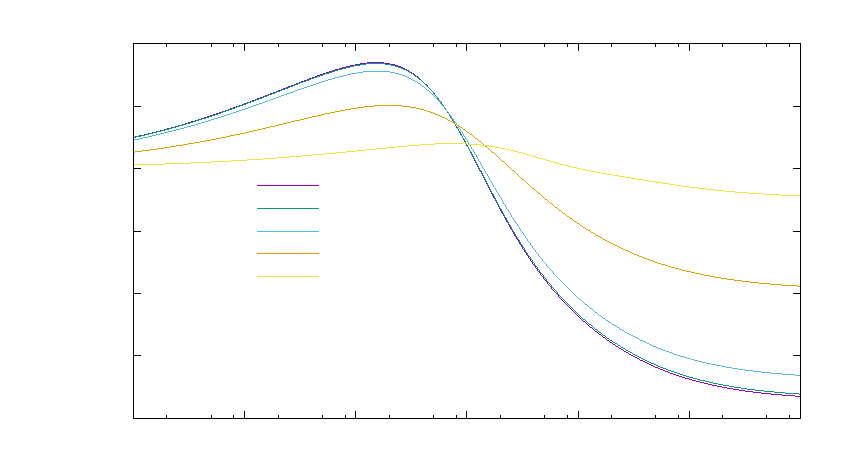
\includegraphics{img/cgBarF1T}}%
    \gplfronttext
  \end{picture}%
\endgroup

	\caption{$\bar c_{T,g}^{F,(1)}(\eta)$}
\end{subfigure}\\%
\begin{subfigure}[t]{\textwidth}
	% GNUPLOT: LaTeX picture with Postscript
\begingroup
  \makeatletter
  \providecommand\color[2][]{%
    \GenericError{(gnuplot) \space\space\space\@spaces}{%
      Package color not loaded in conjunction with
      terminal option `colourtext'%
    }{See the gnuplot documentation for explanation.%
    }{Either use 'blacktext' in gnuplot or load the package
      color.sty in LaTeX.}%
    \renewcommand\color[2][]{}%
  }%
  \providecommand\includegraphics[2][]{%
    \GenericError{(gnuplot) \space\space\space\@spaces}{%
      Package graphicx or graphics not loaded%
    }{See the gnuplot documentation for explanation.%
    }{The gnuplot epslatex terminal needs graphicx.sty or graphics.sty.}%
    \renewcommand\includegraphics[2][]{}%
  }%
  \providecommand\rotatebox[2]{#2}%
  \@ifundefined{ifGPcolor}{%
    \newif\ifGPcolor
    \GPcolorfalse
  }{}%
  \@ifundefined{ifGPblacktext}{%
    \newif\ifGPblacktext
    \GPblacktexttrue
  }{}%
  % define a \g@addto@macro without @ in the name:
  \let\gplgaddtomacro\g@addto@macro
  % define empty templates for all commands taking text:
  \gdef\gplbacktext{}%
  \gdef\gplfronttext{}%
  \makeatother
  \ifGPblacktext
    % no textcolor at all
    \def\colorrgb#1{}%
    \def\colorgray#1{}%
  \else
    % gray or color?
    \ifGPcolor
      \def\colorrgb#1{\color[rgb]{#1}}%
      \def\colorgray#1{\color[gray]{#1}}%
      \expandafter\def\csname LTw\endcsname{\color{white}}%
      \expandafter\def\csname LTb\endcsname{\color{black}}%
      \expandafter\def\csname LTa\endcsname{\color{black}}%
      \expandafter\def\csname LT0\endcsname{\color[rgb]{1,0,0}}%
      \expandafter\def\csname LT1\endcsname{\color[rgb]{0,1,0}}%
      \expandafter\def\csname LT2\endcsname{\color[rgb]{0,0,1}}%
      \expandafter\def\csname LT3\endcsname{\color[rgb]{1,0,1}}%
      \expandafter\def\csname LT4\endcsname{\color[rgb]{0,1,1}}%
      \expandafter\def\csname LT5\endcsname{\color[rgb]{1,1,0}}%
      \expandafter\def\csname LT6\endcsname{\color[rgb]{0,0,0}}%
      \expandafter\def\csname LT7\endcsname{\color[rgb]{1,0.3,0}}%
      \expandafter\def\csname LT8\endcsname{\color[rgb]{0.5,0.5,0.5}}%
    \else
      % gray
      \def\colorrgb#1{\color{black}}%
      \def\colorgray#1{\color[gray]{#1}}%
      \expandafter\def\csname LTw\endcsname{\color{white}}%
      \expandafter\def\csname LTb\endcsname{\color{black}}%
      \expandafter\def\csname LTa\endcsname{\color{black}}%
      \expandafter\def\csname LT0\endcsname{\color{black}}%
      \expandafter\def\csname LT1\endcsname{\color{black}}%
      \expandafter\def\csname LT2\endcsname{\color{black}}%
      \expandafter\def\csname LT3\endcsname{\color{black}}%
      \expandafter\def\csname LT4\endcsname{\color{black}}%
      \expandafter\def\csname LT5\endcsname{\color{black}}%
      \expandafter\def\csname LT6\endcsname{\color{black}}%
      \expandafter\def\csname LT7\endcsname{\color{black}}%
      \expandafter\def\csname LT8\endcsname{\color{black}}%
    \fi
  \fi
    \setlength{\unitlength}{0.0500bp}%
    \ifx\gptboxheight\undefined%
      \newlength{\gptboxheight}%
      \newlength{\gptboxwidth}%
      \newsavebox{\gptboxtext}%
    \fi%
    \setlength{\fboxrule}{0.5pt}%
    \setlength{\fboxsep}{1pt}%
\begin{picture}(7920.00,4082.40)%
    \gplgaddtomacro\gplbacktext{%
      \csname LTb\endcsname%
      \put(990,220){\makebox(0,0)[r]{\strut{}-0.015}}%
      \put(990,940){\makebox(0,0)[r]{\strut{}-0.010}}%
      \put(990,1659){\makebox(0,0)[r]{\strut{}-0.005}}%
      \put(990,2379){\makebox(0,0)[r]{\strut{}0.000}}%
      \put(990,3098){\makebox(0,0)[r]{\strut{}0.005}}%
      \put(990,3818){\makebox(0,0)[r]{\strut{}0.010}}%
      \put(1122,0){\makebox(0,0){\strut{}$0.001$}}%
      \put(2189,0){\makebox(0,0){\strut{}$0.01$}}%
      \put(3255,0){\makebox(0,0){\strut{}$0.1$}}%
      \put(4322,0){\makebox(0,0){\strut{}$1$}}%
      \put(5389,0){\makebox(0,0){\strut{}$10$}}%
      \put(6455,0){\makebox(0,0){\strut{}$100$}}%
      \put(7522,0){\makebox(0,0){\strut{}$1000$}}%
      \put(1250,472){\makebox(0,0)[l]{\strut{}(b) $\bar c_{L,g}^{F,(1)}(\eta)$}}%
    }%
    \gplgaddtomacro\gplfronttext{%
      \csname LTb\endcsname%
      \put(5611,3645){\makebox(0,0)[l]{\strut{}$Q^2=10^{-2}$}}%
      \csname LTb\endcsname%
      \put(5611,3425){\makebox(0,0)[l]{\strut{}$Q^2=10^0$}}%
      \csname LTb\endcsname%
      \put(5611,3205){\makebox(0,0)[l]{\strut{}$Q^2=10^1$}}%
      \csname LTb\endcsname%
      \put(5611,2985){\makebox(0,0)[l]{\strut{}$Q^2=10^2$}}%
      \csname LTb\endcsname%
      \put(5611,2765){\makebox(0,0)[l]{\strut{}$Q^2=10^3$}}%
    }%
    \gplbacktext
    \put(0,0){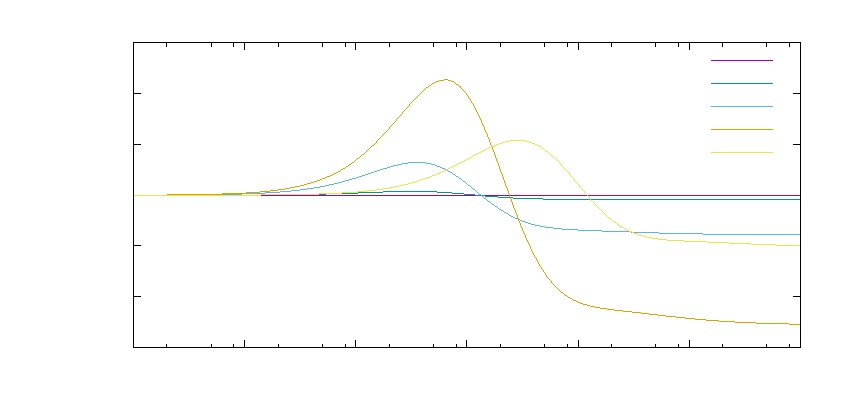
\includegraphics{img/cgBarF1L}}%
    \gplfronttext
  \end{picture}%
\endgroup

	\caption{$\bar c_{L,g}^{F,(1)}(\eta)$}
\end{subfigure}\\%
\begin{subfigure}[t]{\textwidth}
	% GNUPLOT: LaTeX picture with Postscript
\begingroup
  \makeatletter
  \providecommand\color[2][]{%
    \GenericError{(gnuplot) \space\space\space\@spaces}{%
      Package color not loaded in conjunction with
      terminal option `colourtext'%
    }{See the gnuplot documentation for explanation.%
    }{Either use 'blacktext' in gnuplot or load the package
      color.sty in LaTeX.}%
    \renewcommand\color[2][]{}%
  }%
  \providecommand\includegraphics[2][]{%
    \GenericError{(gnuplot) \space\space\space\@spaces}{%
      Package graphicx or graphics not loaded%
    }{See the gnuplot documentation for explanation.%
    }{The gnuplot epslatex terminal needs graphicx.sty or graphics.sty.}%
    \renewcommand\includegraphics[2][]{}%
  }%
  \providecommand\rotatebox[2]{#2}%
  \@ifundefined{ifGPcolor}{%
    \newif\ifGPcolor
    \GPcolorfalse
  }{}%
  \@ifundefined{ifGPblacktext}{%
    \newif\ifGPblacktext
    \GPblacktexttrue
  }{}%
  % define a \g@addto@macro without @ in the name:
  \let\gplgaddtomacro\g@addto@macro
  % define empty templates for all commands taking text:
  \gdef\gplbacktext{}%
  \gdef\gplfronttext{}%
  \makeatother
  \ifGPblacktext
    % no textcolor at all
    \def\colorrgb#1{}%
    \def\colorgray#1{}%
  \else
    % gray or color?
    \ifGPcolor
      \def\colorrgb#1{\color[rgb]{#1}}%
      \def\colorgray#1{\color[gray]{#1}}%
      \expandafter\def\csname LTw\endcsname{\color{white}}%
      \expandafter\def\csname LTb\endcsname{\color{black}}%
      \expandafter\def\csname LTa\endcsname{\color{black}}%
      \expandafter\def\csname LT0\endcsname{\color[rgb]{1,0,0}}%
      \expandafter\def\csname LT1\endcsname{\color[rgb]{0,1,0}}%
      \expandafter\def\csname LT2\endcsname{\color[rgb]{0,0,1}}%
      \expandafter\def\csname LT3\endcsname{\color[rgb]{1,0,1}}%
      \expandafter\def\csname LT4\endcsname{\color[rgb]{0,1,1}}%
      \expandafter\def\csname LT5\endcsname{\color[rgb]{1,1,0}}%
      \expandafter\def\csname LT6\endcsname{\color[rgb]{0,0,0}}%
      \expandafter\def\csname LT7\endcsname{\color[rgb]{1,0.3,0}}%
      \expandafter\def\csname LT8\endcsname{\color[rgb]{0.5,0.5,0.5}}%
    \else
      % gray
      \def\colorrgb#1{\color{black}}%
      \def\colorgray#1{\color[gray]{#1}}%
      \expandafter\def\csname LTw\endcsname{\color{white}}%
      \expandafter\def\csname LTb\endcsname{\color{black}}%
      \expandafter\def\csname LTa\endcsname{\color{black}}%
      \expandafter\def\csname LT0\endcsname{\color{black}}%
      \expandafter\def\csname LT1\endcsname{\color{black}}%
      \expandafter\def\csname LT2\endcsname{\color{black}}%
      \expandafter\def\csname LT3\endcsname{\color{black}}%
      \expandafter\def\csname LT4\endcsname{\color{black}}%
      \expandafter\def\csname LT5\endcsname{\color{black}}%
      \expandafter\def\csname LT6\endcsname{\color{black}}%
      \expandafter\def\csname LT7\endcsname{\color{black}}%
      \expandafter\def\csname LT8\endcsname{\color{black}}%
    \fi
  \fi
    \setlength{\unitlength}{0.0500bp}%
    \ifx\gptboxheight\undefined%
      \newlength{\gptboxheight}%
      \newlength{\gptboxwidth}%
      \newsavebox{\gptboxtext}%
    \fi%
    \setlength{\fboxrule}{0.5pt}%
    \setlength{\fboxsep}{1pt}%
\begin{picture}(7920.00,4082.40)%
    \gplgaddtomacro\gplbacktext{%
      \csname LTb\endcsname%
      \put(990,220){\makebox(0,0)[r]{\strut{} -0.04}}%
      \put(990,580){\makebox(0,0)[r]{\strut{} -0.03}}%
      \put(990,940){\makebox(0,0)[r]{\strut{} -0.02}}%
      \put(990,1299){\makebox(0,0)[r]{\strut{} -0.01}}%
      \put(990,1659){\makebox(0,0)[r]{\strut{} 0.00}}%
      \put(990,2019){\makebox(0,0)[r]{\strut{} 0.01}}%
      \put(990,2379){\makebox(0,0)[r]{\strut{} 0.02}}%
      \put(990,2739){\makebox(0,0)[r]{\strut{} 0.03}}%
      \put(990,3098){\makebox(0,0)[r]{\strut{} 0.04}}%
      \put(990,3458){\makebox(0,0)[r]{\strut{} 0.05}}%
      \put(990,3818){\makebox(0,0)[r]{\strut{} 0.06}}%
      \put(1122,0){\makebox(0,0){\strut{}$0.001$}}%
      \put(2189,0){\makebox(0,0){\strut{}$0.01$}}%
      \put(3255,0){\makebox(0,0){\strut{}$0.1$}}%
      \put(4322,0){\makebox(0,0){\strut{}$1$}}%
      \put(5389,0){\makebox(0,0){\strut{}$10$}}%
      \put(6455,0){\makebox(0,0){\strut{}$100$}}%
      \put(7522,0){\makebox(0,0){\strut{}$1000$}}%
      \put(1250,472){\makebox(0,0)[l]{\strut{}(c) $\bar c_{P,g}^{F,(1)}(\eta)$}}%
    }%
    \gplgaddtomacro\gplfronttext{%
      \csname LTb\endcsname%
      \put(5611,3645){\makebox(0,0)[l]{\strut{}$Q^2=10^{-2}$}}%
      \csname LTb\endcsname%
      \put(5611,3425){\makebox(0,0)[l]{\strut{}$Q^2=10^0$}}%
      \csname LTb\endcsname%
      \put(5611,3205){\makebox(0,0)[l]{\strut{}$Q^2=10^1$}}%
      \csname LTb\endcsname%
      \put(5611,2985){\makebox(0,0)[l]{\strut{}$Q^2=10^2$}}%
      \csname LTb\endcsname%
      \put(5611,2765){\makebox(0,0)[l]{\strut{}$Q^2=10^3$}}%
    }%
    \gplbacktext
    \put(0,0){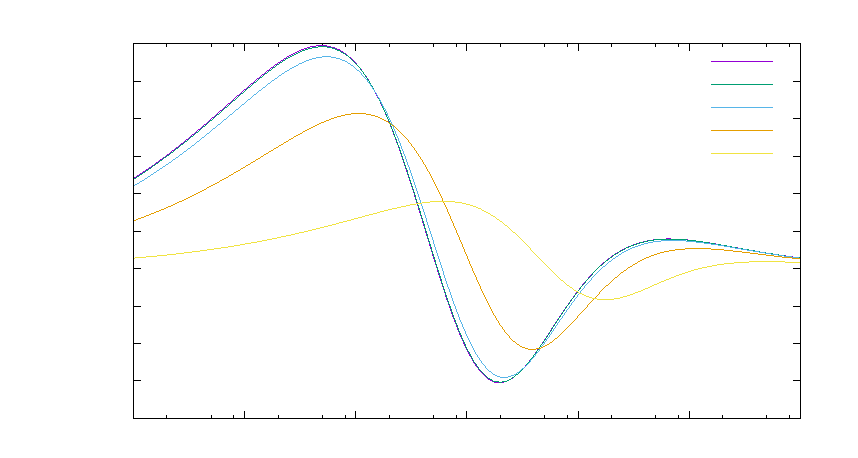
\includegraphics{img/cgBarF1P}}%
    \gplfronttext
  \end{picture}%
\endgroup

	\caption{$\bar c_{P,g}^{F,(1)}(\eta)$}
\end{subfigure}
\caption{next-to-leading order scaling functions $\bar c_{k,g}^{F,(1)}(\eta,\xi)$ plotted as function of $\eta=s/(4m^2)-1$ for different values of $Q^2$ in units of $\si{\GeV^2}$ at $m=\SI{4.75}{\GeV}$ (i.e. different values of $\xi=Q^2/m^2$) and $n_{lf}=4$ }\label{fig:cg1}
\end{figure}

\pagebreak
\begin{figure}[ht!]
\centering
\begin{subfigure}[t]{\textwidth}
	% GNUPLOT: LaTeX picture with Postscript
\begingroup
  \makeatletter
  \providecommand\color[2][]{%
    \GenericError{(gnuplot) \space\space\space\@spaces}{%
      Package color not loaded in conjunction with
      terminal option `colourtext'%
    }{See the gnuplot documentation for explanation.%
    }{Either use 'blacktext' in gnuplot or load the package
      color.sty in LaTeX.}%
    \renewcommand\color[2][]{}%
  }%
  \providecommand\includegraphics[2][]{%
    \GenericError{(gnuplot) \space\space\space\@spaces}{%
      Package graphicx or graphics not loaded%
    }{See the gnuplot documentation for explanation.%
    }{The gnuplot epslatex terminal needs graphicx.sty or graphics.sty.}%
    \renewcommand\includegraphics[2][]{}%
  }%
  \providecommand\rotatebox[2]{#2}%
  \@ifundefined{ifGPcolor}{%
    \newif\ifGPcolor
    \GPcolorfalse
  }{}%
  \@ifundefined{ifGPblacktext}{%
    \newif\ifGPblacktext
    \GPblacktexttrue
  }{}%
  % define a \g@addto@macro without @ in the name:
  \let\gplgaddtomacro\g@addto@macro
  % define empty templates for all commands taking text:
  \gdef\gplbacktext{}%
  \gdef\gplfronttext{}%
  \makeatother
  \ifGPblacktext
    % no textcolor at all
    \def\colorrgb#1{}%
    \def\colorgray#1{}%
  \else
    % gray or color?
    \ifGPcolor
      \def\colorrgb#1{\color[rgb]{#1}}%
      \def\colorgray#1{\color[gray]{#1}}%
      \expandafter\def\csname LTw\endcsname{\color{white}}%
      \expandafter\def\csname LTb\endcsname{\color{black}}%
      \expandafter\def\csname LTa\endcsname{\color{black}}%
      \expandafter\def\csname LT0\endcsname{\color[rgb]{1,0,0}}%
      \expandafter\def\csname LT1\endcsname{\color[rgb]{0,1,0}}%
      \expandafter\def\csname LT2\endcsname{\color[rgb]{0,0,1}}%
      \expandafter\def\csname LT3\endcsname{\color[rgb]{1,0,1}}%
      \expandafter\def\csname LT4\endcsname{\color[rgb]{0,1,1}}%
      \expandafter\def\csname LT5\endcsname{\color[rgb]{1,1,0}}%
      \expandafter\def\csname LT6\endcsname{\color[rgb]{0,0,0}}%
      \expandafter\def\csname LT7\endcsname{\color[rgb]{1,0.3,0}}%
      \expandafter\def\csname LT8\endcsname{\color[rgb]{0.5,0.5,0.5}}%
    \else
      % gray
      \def\colorrgb#1{\color{black}}%
      \def\colorgray#1{\color[gray]{#1}}%
      \expandafter\def\csname LTw\endcsname{\color{white}}%
      \expandafter\def\csname LTb\endcsname{\color{black}}%
      \expandafter\def\csname LTa\endcsname{\color{black}}%
      \expandafter\def\csname LT0\endcsname{\color{black}}%
      \expandafter\def\csname LT1\endcsname{\color{black}}%
      \expandafter\def\csname LT2\endcsname{\color{black}}%
      \expandafter\def\csname LT3\endcsname{\color{black}}%
      \expandafter\def\csname LT4\endcsname{\color{black}}%
      \expandafter\def\csname LT5\endcsname{\color{black}}%
      \expandafter\def\csname LT6\endcsname{\color{black}}%
      \expandafter\def\csname LT7\endcsname{\color{black}}%
      \expandafter\def\csname LT8\endcsname{\color{black}}%
    \fi
  \fi
    \setlength{\unitlength}{0.0500bp}%
    \ifx\gptboxheight\undefined%
      \newlength{\gptboxheight}%
      \newlength{\gptboxwidth}%
      \newsavebox{\gptboxtext}%
    \fi%
    \setlength{\fboxrule}{0.5pt}%
    \setlength{\fboxsep}{1pt}%
\begin{picture}(7920.00,4082.40)%
    \gplgaddtomacro\gplbacktext{%
      \csname LTb\endcsname%
      \put(726,220){\makebox(0,0)[r]{\strut{}0.00}}%
      \put(726,580){\makebox(0,0)[r]{\strut{}0.01}}%
      \put(726,940){\makebox(0,0)[r]{\strut{}0.02}}%
      \put(726,1299){\makebox(0,0)[r]{\strut{}0.03}}%
      \put(726,1659){\makebox(0,0)[r]{\strut{}0.04}}%
      \put(726,2019){\makebox(0,0)[r]{\strut{}0.05}}%
      \put(726,2379){\makebox(0,0)[r]{\strut{}0.06}}%
      \put(726,2739){\makebox(0,0)[r]{\strut{}0.07}}%
      \put(726,3098){\makebox(0,0)[r]{\strut{}0.08}}%
      \put(726,3458){\makebox(0,0)[r]{\strut{}0.09}}%
      \put(726,3818){\makebox(0,0)[r]{\strut{}0.10}}%
      \put(858,0){\makebox(0,0){\strut{}$0.001$}}%
      \put(1969,0){\makebox(0,0){\strut{}$0.01$}}%
      \put(3079,0){\makebox(0,0){\strut{}$0.1$}}%
      \put(4190,0){\makebox(0,0){\strut{}$1$}}%
      \put(5301,0){\makebox(0,0){\strut{}$10$}}%
      \put(6411,0){\makebox(0,0){\strut{}$100$}}%
      \put(7522,0){\makebox(0,0){\strut{}$1000$}}%
      \put(991,3458){\makebox(0,0)[l]{\strut{}(a) $\bar c_{T,g}^{R,(1)}(\eta)$}}%
    }%
    \gplgaddtomacro\gplfronttext{%
      \csname LTb\endcsname%
      \put(5611,3645){\makebox(0,0)[l]{\strut{}$Q^2=10^{-2}$}}%
      \csname LTb\endcsname%
      \put(5611,3425){\makebox(0,0)[l]{\strut{}$Q^2=10^0$}}%
      \csname LTb\endcsname%
      \put(5611,3205){\makebox(0,0)[l]{\strut{}$Q^2=10^1$}}%
      \csname LTb\endcsname%
      \put(5611,2985){\makebox(0,0)[l]{\strut{}$Q^2=10^2$}}%
      \csname LTb\endcsname%
      \put(5611,2765){\makebox(0,0)[l]{\strut{}$Q^2=10^3$}}%
    }%
    \gplbacktext
    \put(0,0){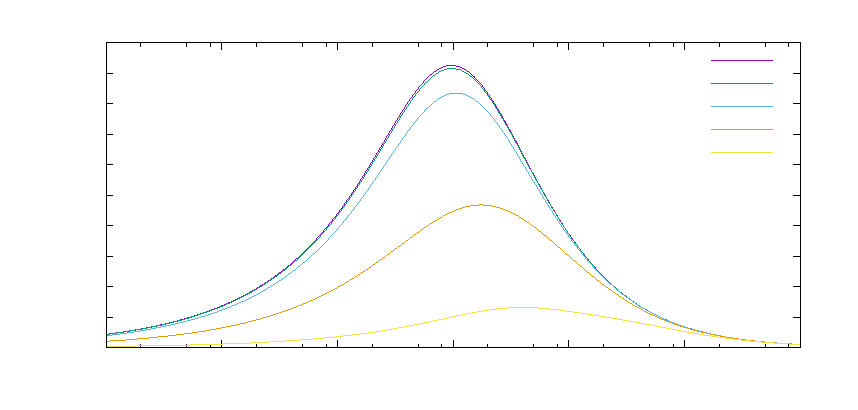
\includegraphics{img/cgBarR1T}}%
    \gplfronttext
  \end{picture}%
\endgroup

	\caption{$\bar c_{T,g}^{R,(1)}(\eta)$}
\end{subfigure}\\%
\begin{subfigure}[t]{\textwidth}
	% GNUPLOT: LaTeX picture with Postscript
\begingroup
  \makeatletter
  \providecommand\color[2][]{%
    \GenericError{(gnuplot) \space\space\space\@spaces}{%
      Package color not loaded in conjunction with
      terminal option `colourtext'%
    }{See the gnuplot documentation for explanation.%
    }{Either use 'blacktext' in gnuplot or load the package
      color.sty in LaTeX.}%
    \renewcommand\color[2][]{}%
  }%
  \providecommand\includegraphics[2][]{%
    \GenericError{(gnuplot) \space\space\space\@spaces}{%
      Package graphicx or graphics not loaded%
    }{See the gnuplot documentation for explanation.%
    }{The gnuplot epslatex terminal needs graphicx.sty or graphics.sty.}%
    \renewcommand\includegraphics[2][]{}%
  }%
  \providecommand\rotatebox[2]{#2}%
  \@ifundefined{ifGPcolor}{%
    \newif\ifGPcolor
    \GPcolorfalse
  }{}%
  \@ifundefined{ifGPblacktext}{%
    \newif\ifGPblacktext
    \GPblacktexttrue
  }{}%
  % define a \g@addto@macro without @ in the name:
  \let\gplgaddtomacro\g@addto@macro
  % define empty templates for all commands taking text:
  \gdef\gplbacktext{}%
  \gdef\gplfronttext{}%
  \makeatother
  \ifGPblacktext
    % no textcolor at all
    \def\colorrgb#1{}%
    \def\colorgray#1{}%
  \else
    % gray or color?
    \ifGPcolor
      \def\colorrgb#1{\color[rgb]{#1}}%
      \def\colorgray#1{\color[gray]{#1}}%
      \expandafter\def\csname LTw\endcsname{\color{white}}%
      \expandafter\def\csname LTb\endcsname{\color{black}}%
      \expandafter\def\csname LTa\endcsname{\color{black}}%
      \expandafter\def\csname LT0\endcsname{\color[rgb]{1,0,0}}%
      \expandafter\def\csname LT1\endcsname{\color[rgb]{0,1,0}}%
      \expandafter\def\csname LT2\endcsname{\color[rgb]{0,0,1}}%
      \expandafter\def\csname LT3\endcsname{\color[rgb]{1,0,1}}%
      \expandafter\def\csname LT4\endcsname{\color[rgb]{0,1,1}}%
      \expandafter\def\csname LT5\endcsname{\color[rgb]{1,1,0}}%
      \expandafter\def\csname LT6\endcsname{\color[rgb]{0,0,0}}%
      \expandafter\def\csname LT7\endcsname{\color[rgb]{1,0.3,0}}%
      \expandafter\def\csname LT8\endcsname{\color[rgb]{0.5,0.5,0.5}}%
    \else
      % gray
      \def\colorrgb#1{\color{black}}%
      \def\colorgray#1{\color[gray]{#1}}%
      \expandafter\def\csname LTw\endcsname{\color{white}}%
      \expandafter\def\csname LTb\endcsname{\color{black}}%
      \expandafter\def\csname LTa\endcsname{\color{black}}%
      \expandafter\def\csname LT0\endcsname{\color{black}}%
      \expandafter\def\csname LT1\endcsname{\color{black}}%
      \expandafter\def\csname LT2\endcsname{\color{black}}%
      \expandafter\def\csname LT3\endcsname{\color{black}}%
      \expandafter\def\csname LT4\endcsname{\color{black}}%
      \expandafter\def\csname LT5\endcsname{\color{black}}%
      \expandafter\def\csname LT6\endcsname{\color{black}}%
      \expandafter\def\csname LT7\endcsname{\color{black}}%
      \expandafter\def\csname LT8\endcsname{\color{black}}%
    \fi
  \fi
    \setlength{\unitlength}{0.0500bp}%
    \ifx\gptboxheight\undefined%
      \newlength{\gptboxheight}%
      \newlength{\gptboxwidth}%
      \newsavebox{\gptboxtext}%
    \fi%
    \setlength{\fboxrule}{0.5pt}%
    \setlength{\fboxsep}{1pt}%
\begin{picture}(7920.00,3628.80)%
    \gplgaddtomacro\gplbacktext{%
      \csname LTb\endcsname%
      \put(858,440){\makebox(0,0)[r]{\strut{}0.000}}%
      \put(858,927){\makebox(0,0)[r]{\strut{}0.002}}%
      \put(858,1415){\makebox(0,0)[r]{\strut{}0.004}}%
      \put(858,1902){\makebox(0,0)[r]{\strut{}0.006}}%
      \put(858,2389){\makebox(0,0)[r]{\strut{}0.008}}%
      \put(858,2877){\makebox(0,0)[r]{\strut{}0.010}}%
      \put(858,3364){\makebox(0,0)[r]{\strut{}0.012}}%
      \put(990,220){\makebox(0,0){\strut{}$0.001$}}%
      \put(2079,220){\makebox(0,0){\strut{}$0.01$}}%
      \put(3167,220){\makebox(0,0){\strut{}$0.1$}}%
      \put(4256,220){\makebox(0,0){\strut{}$1$}}%
      \put(5345,220){\makebox(0,0){\strut{}$10$}}%
      \put(6433,220){\makebox(0,0){\strut{}$100$}}%
      \put(7522,220){\makebox(0,0){\strut{}$1000$}}%
    }%
    \gplgaddtomacro\gplfronttext{%
      \csname LTb\endcsname%
      \put(5611,3191){\makebox(0,0)[l]{\strut{}$Q^2=10^{-2}$}}%
      \csname LTb\endcsname%
      \put(5611,2971){\makebox(0,0)[l]{\strut{}$Q^2=10^0$}}%
      \csname LTb\endcsname%
      \put(5611,2751){\makebox(0,0)[l]{\strut{}$Q^2=10^1$}}%
      \csname LTb\endcsname%
      \put(5611,2531){\makebox(0,0)[l]{\strut{}$Q^2=10^2$}}%
      \csname LTb\endcsname%
      \put(5611,2311){\makebox(0,0)[l]{\strut{}$Q^2=10^3$}}%
    }%
    \gplbacktext
    \put(0,0){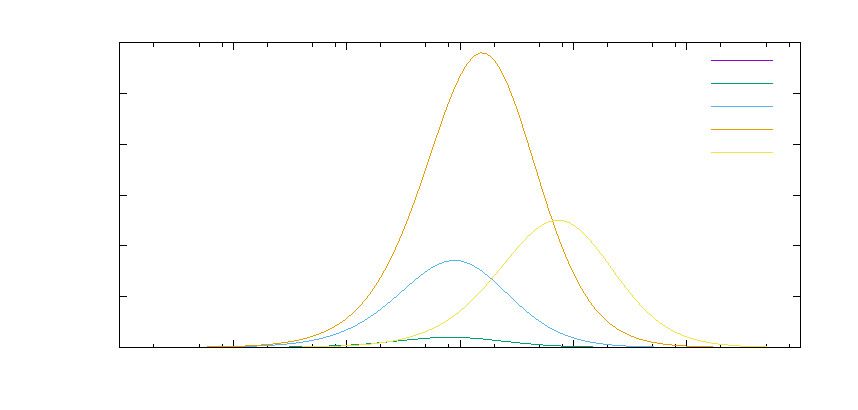
\includegraphics{img/cgBarR1L}}%
    \gplfronttext
  \end{picture}%
\endgroup

	\caption{$\bar c_{L,g}^{R,(1)}(\eta)$}
\end{subfigure}\\%
\begin{subfigure}[t]{\textwidth}
	% GNUPLOT: LaTeX picture with Postscript
\begingroup
  \makeatletter
  \providecommand\color[2][]{%
    \GenericError{(gnuplot) \space\space\space\@spaces}{%
      Package color not loaded in conjunction with
      terminal option `colourtext'%
    }{See the gnuplot documentation for explanation.%
    }{Either use 'blacktext' in gnuplot or load the package
      color.sty in LaTeX.}%
    \renewcommand\color[2][]{}%
  }%
  \providecommand\includegraphics[2][]{%
    \GenericError{(gnuplot) \space\space\space\@spaces}{%
      Package graphicx or graphics not loaded%
    }{See the gnuplot documentation for explanation.%
    }{The gnuplot epslatex terminal needs graphicx.sty or graphics.sty.}%
    \renewcommand\includegraphics[2][]{}%
  }%
  \providecommand\rotatebox[2]{#2}%
  \@ifundefined{ifGPcolor}{%
    \newif\ifGPcolor
    \GPcolorfalse
  }{}%
  \@ifundefined{ifGPblacktext}{%
    \newif\ifGPblacktext
    \GPblacktexttrue
  }{}%
  % define a \g@addto@macro without @ in the name:
  \let\gplgaddtomacro\g@addto@macro
  % define empty templates for all commands taking text:
  \gdef\gplbacktext{}%
  \gdef\gplfronttext{}%
  \makeatother
  \ifGPblacktext
    % no textcolor at all
    \def\colorrgb#1{}%
    \def\colorgray#1{}%
  \else
    % gray or color?
    \ifGPcolor
      \def\colorrgb#1{\color[rgb]{#1}}%
      \def\colorgray#1{\color[gray]{#1}}%
      \expandafter\def\csname LTw\endcsname{\color{white}}%
      \expandafter\def\csname LTb\endcsname{\color{black}}%
      \expandafter\def\csname LTa\endcsname{\color{black}}%
      \expandafter\def\csname LT0\endcsname{\color[rgb]{1,0,0}}%
      \expandafter\def\csname LT1\endcsname{\color[rgb]{0,1,0}}%
      \expandafter\def\csname LT2\endcsname{\color[rgb]{0,0,1}}%
      \expandafter\def\csname LT3\endcsname{\color[rgb]{1,0,1}}%
      \expandafter\def\csname LT4\endcsname{\color[rgb]{0,1,1}}%
      \expandafter\def\csname LT5\endcsname{\color[rgb]{1,1,0}}%
      \expandafter\def\csname LT6\endcsname{\color[rgb]{0,0,0}}%
      \expandafter\def\csname LT7\endcsname{\color[rgb]{1,0.3,0}}%
      \expandafter\def\csname LT8\endcsname{\color[rgb]{0.5,0.5,0.5}}%
    \else
      % gray
      \def\colorrgb#1{\color{black}}%
      \def\colorgray#1{\color[gray]{#1}}%
      \expandafter\def\csname LTw\endcsname{\color{white}}%
      \expandafter\def\csname LTb\endcsname{\color{black}}%
      \expandafter\def\csname LTa\endcsname{\color{black}}%
      \expandafter\def\csname LT0\endcsname{\color{black}}%
      \expandafter\def\csname LT1\endcsname{\color{black}}%
      \expandafter\def\csname LT2\endcsname{\color{black}}%
      \expandafter\def\csname LT3\endcsname{\color{black}}%
      \expandafter\def\csname LT4\endcsname{\color{black}}%
      \expandafter\def\csname LT5\endcsname{\color{black}}%
      \expandafter\def\csname LT6\endcsname{\color{black}}%
      \expandafter\def\csname LT7\endcsname{\color{black}}%
      \expandafter\def\csname LT8\endcsname{\color{black}}%
    \fi
  \fi
    \setlength{\unitlength}{0.0500bp}%
    \ifx\gptboxheight\undefined%
      \newlength{\gptboxheight}%
      \newlength{\gptboxwidth}%
      \newsavebox{\gptboxtext}%
    \fi%
    \setlength{\fboxrule}{0.5pt}%
    \setlength{\fboxsep}{1pt}%
\begin{picture}(7920.00,4082.40)%
    \gplgaddtomacro\gplbacktext{%
      \csname LTb\endcsname%
      \put(858,220){\makebox(0,0)[r]{\strut{}-0.02}}%
      \put(858,734){\makebox(0,0)[r]{\strut{}-0.01}}%
      \put(858,1248){\makebox(0,0)[r]{\strut{}0.00}}%
      \put(858,1762){\makebox(0,0)[r]{\strut{}0.01}}%
      \put(858,2276){\makebox(0,0)[r]{\strut{}0.02}}%
      \put(858,2790){\makebox(0,0)[r]{\strut{}0.03}}%
      \put(858,3304){\makebox(0,0)[r]{\strut{}0.04}}%
      \put(858,3818){\makebox(0,0)[r]{\strut{}0.05}}%
      \put(990,0){\makebox(0,0){\strut{}$0.001$}}%
      \put(2079,0){\makebox(0,0){\strut{}$0.01$}}%
      \put(3167,0){\makebox(0,0){\strut{}$0.1$}}%
      \put(4256,0){\makebox(0,0){\strut{}$1$}}%
      \put(5345,0){\makebox(0,0){\strut{}$10$}}%
      \put(6433,0){\makebox(0,0){\strut{}$100$}}%
      \put(7522,0){\makebox(0,0){\strut{}$1000$}}%
      \put(1121,3458){\makebox(0,0)[l]{\strut{}(c) $\bar c_{P,g}^{R,(1)}(\eta)$}}%
    }%
    \gplgaddtomacro\gplfronttext{%
      \csname LTb\endcsname%
      \put(5611,3645){\makebox(0,0)[l]{\strut{}$Q^2=10^{-2}$}}%
      \csname LTb\endcsname%
      \put(5611,3425){\makebox(0,0)[l]{\strut{}$Q^2=10^0$}}%
      \csname LTb\endcsname%
      \put(5611,3205){\makebox(0,0)[l]{\strut{}$Q^2=10^1$}}%
      \csname LTb\endcsname%
      \put(5611,2985){\makebox(0,0)[l]{\strut{}$Q^2=10^2$}}%
      \csname LTb\endcsname%
      \put(5611,2765){\makebox(0,0)[l]{\strut{}$Q^2=10^3$}}%
    }%
    \gplbacktext
    \put(0,0){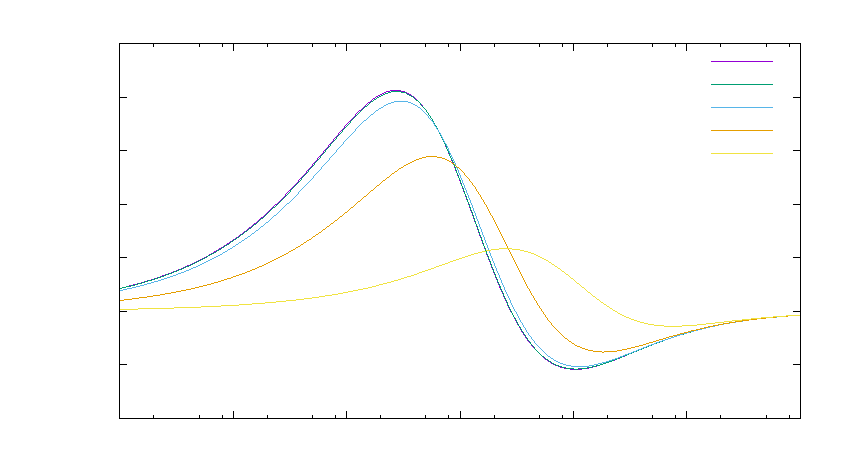
\includegraphics{img/cgBarR1P}}%
    \gplfronttext
  \end{picture}%
\endgroup

	\caption{$\bar c_{P,g}^{R,(1)}(\eta)$}
\end{subfigure}
\caption{next-to-leading order scaling functions $\bar c_{k,g}^{R,(1)}(\eta,\xi)$ plotted as function of $\eta=s/(4m^2)-1$ for different values of $Q^2$ in units of $\si{\GeV^2}$ at $m=\SI{4.75}{\GeV}$ (i.e. different values of $\xi=Q^2/m^2$) and $n_{lf}=4$ }\label{fig:cg1}
\end{figure}

\clearpage


\section{Hadronic Results}
\section{Hadronic Results}
\begin{frame}{Hadronic Results - Unpolarized vs. Polarized}
\begin{center}
unpolarized $\sim$ MSTW2008 $\leftrightarrow$ polarized $\sim$ DSSV2014\quad\,\,\,\\
\quad\quad\quad\iRef{Martin,Stirling,Thorne,Watt} $\leftrightarrow$ \iRef{de Florian,Sassot,Stratmann,Vogelsang}
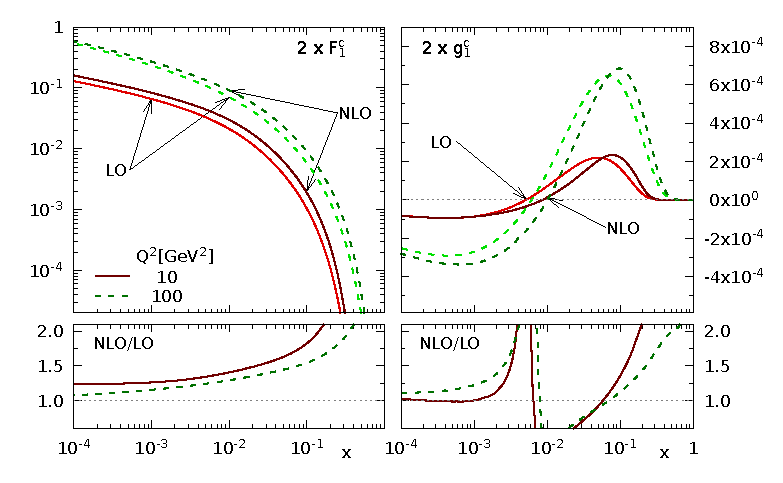
\includegraphics[width=.8\textwidth]{img/F1g1}
\end{center}
\end{frame}

\begin{frame}{Hadronic Results - PDF Uncertainties DSSV (I)}
\newcolumntype{w}{>{\centering\arraybackslash} m{.60\linewidth} }
\newcolumntype{n}{>{\centering\arraybackslash} m{.39\linewidth} }
\begin{tabular}{wn}
\begin{center}
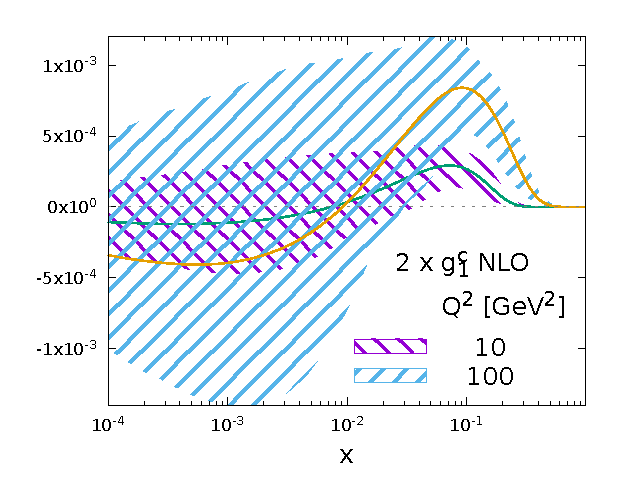
\includegraphics[width=.65\textwidth]{img/g1NLO-pdf}
\end{center} & 
\begin{itemize}
\item quark error band is small
\item sign unconstrained
\item gluon dominates (?)
\item default gluon is small
\end{itemize}
\end{tabular}
\end{frame}

\begin{frame}{Hadronic Results - PDF Uncertainties DSSV (II)}
\newcolumntype{w}{>{\centering\arraybackslash} m{.5\linewidth} }
\newcolumntype{n}{>{\centering\arraybackslash} m{.5\linewidth} }
\begin{tabular}{wn}
\begin{center}
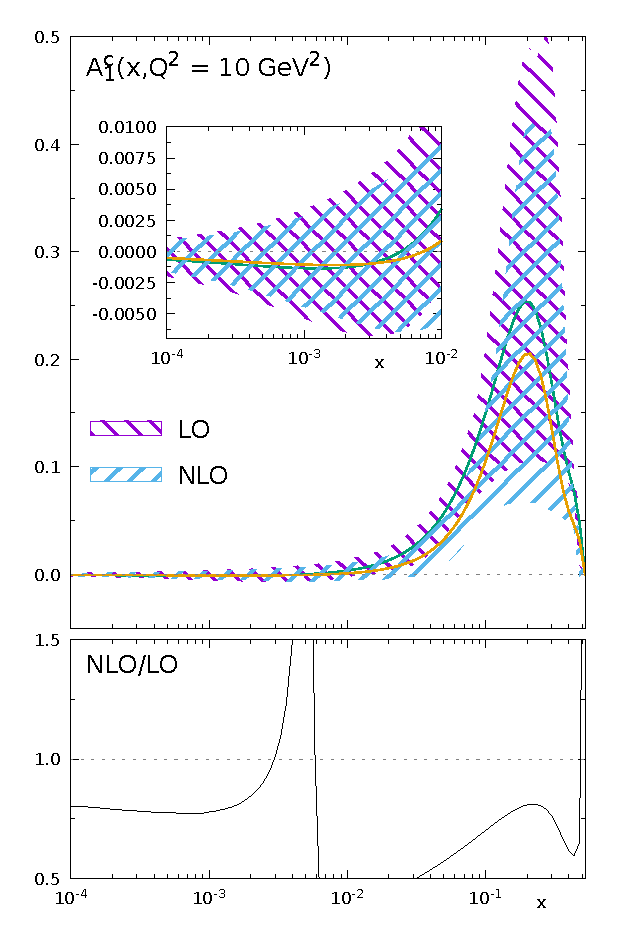
\includegraphics[height=.97\textheight]{img/A1-pdf}
\end{center} & 
\begin{itemize}
\item $A_1^c(x,Q^2) = \frac{g_1^c(x,Q^2)}{F_1^c(x,Q^2)}$
\item error band are only due to DSSV uncertainties (no correlations!)
\invisible{
\item sign unconstrained
\item need measurement of $\mathcal O(10^{-3})$
\item NLO $\lessapprox$ LO}
\end{itemize}
\end{tabular}
\end{frame}
\begin{frame}{Hadronic Results - PDF Uncertainties DSSV (II)}
\newcolumntype{w}{>{\centering\arraybackslash} m{.5\linewidth} }
\newcolumntype{n}{>{\centering\arraybackslash} m{.5\linewidth} }
\begin{tabular}{wn}
\begin{center}
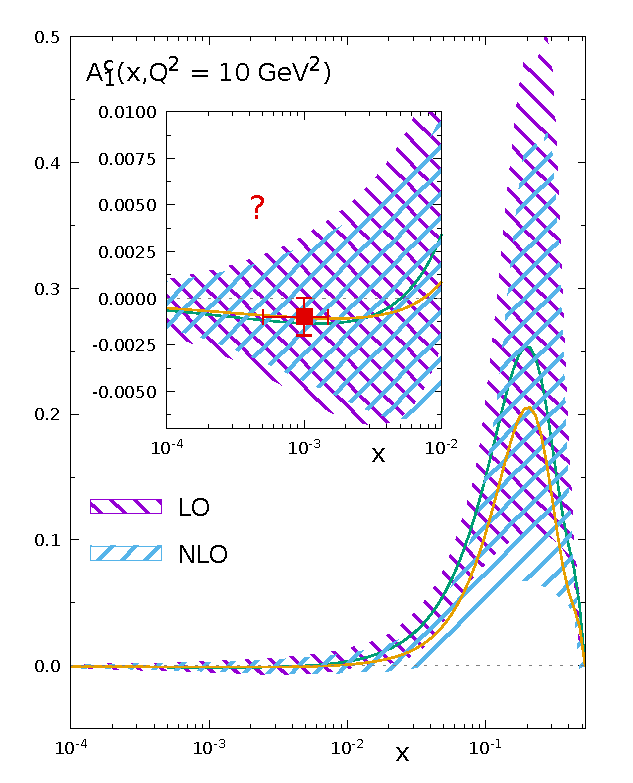
\includegraphics[height=.97\textheight]{img/A1-pdf-data}
\end{center} & 
\begin{itemize}
\item $A_1^c(x,Q^2) = \frac{g_1^c(x,Q^2)}{F_1^c(x,Q^2)}$
\item error band are only due to DSSV uncertainties (no correlations!)
\item sign unconstrained
\item need measurement of $\mathcal O(10^{-3})$
\item NLO $\lessapprox$ LO
\end{itemize}
\end{tabular}
\end{frame}

\begin{frame}{Hadronic Results - Scale Uncertainties (I)}
\begin{center}
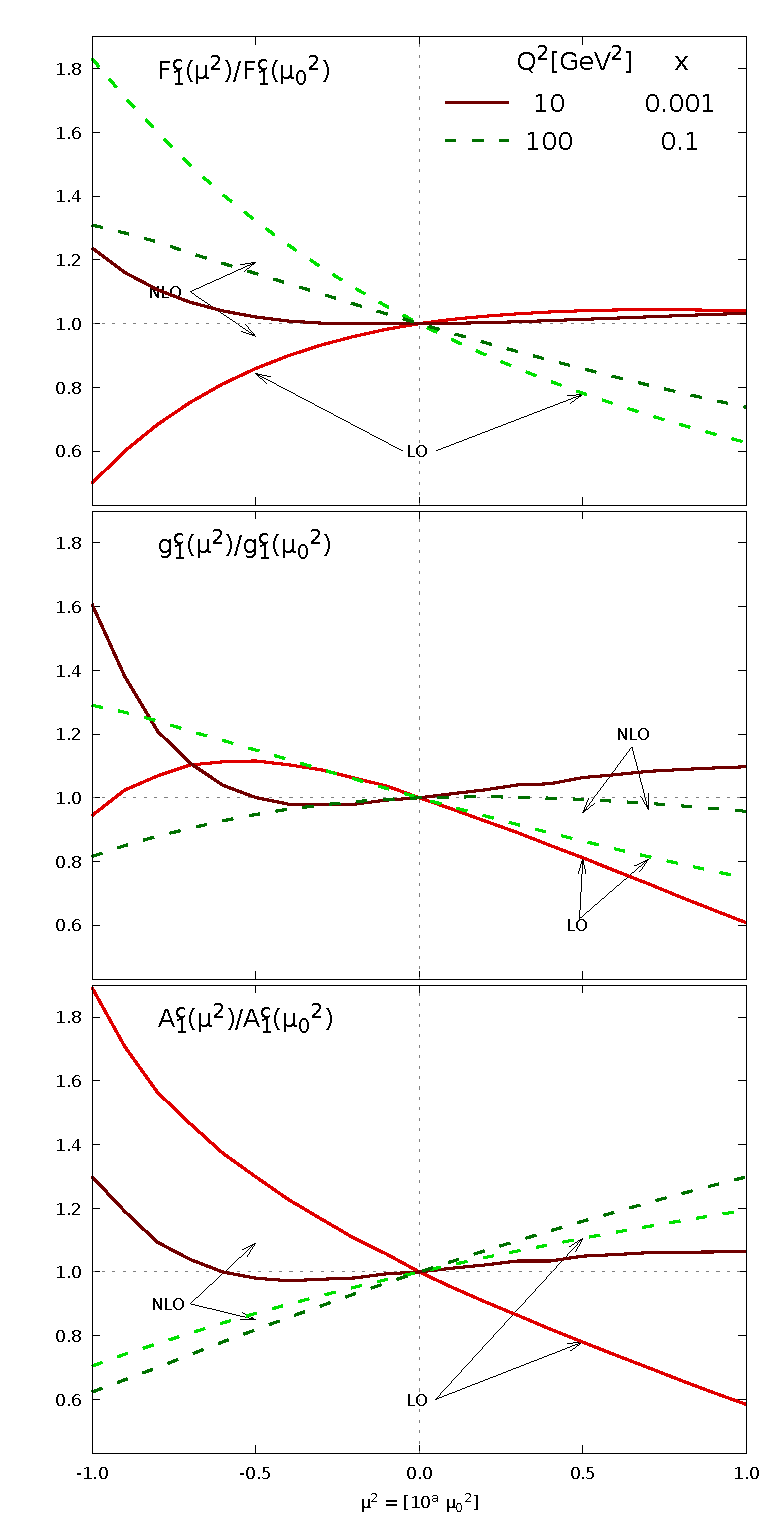
\includegraphics[width=\textwidth]{img/F1g1A1-mu2}
\end{center}
\[\mu_F^2 = \mu_R^2 = 10^a\mu_0^2\,\text{with}\,\mu_0^2=4m^2+Q^2\]
\end{frame}

\begin{frame}{Hadronic Results - Scale Uncertainties (II)}
\begin{center}
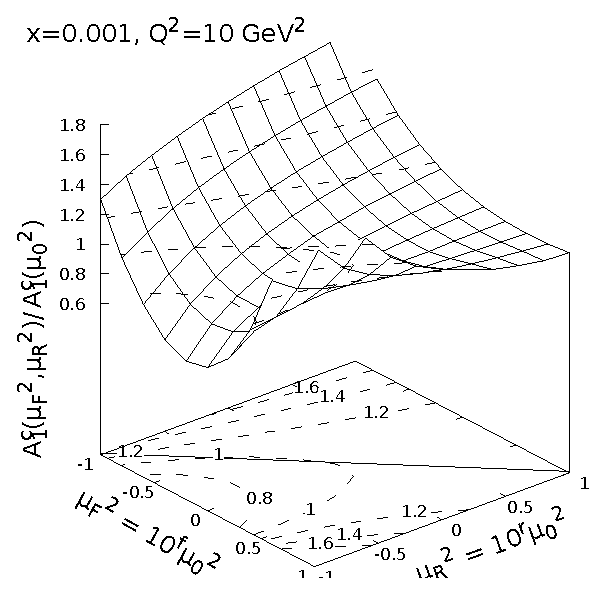
\includegraphics[width=.48\textwidth]{img/A1-muF2-muR2-x_3-q2_1}
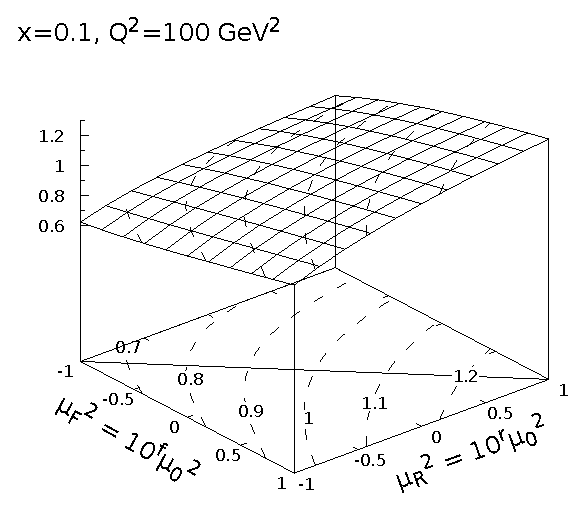
\includegraphics[width=.48\textwidth]{img/A1-muF2-muR2-x_1-q2_2}
\end{center}
\[\mu_0^2=4m^2+Q^2\]
\end{frame}


\section{Summary}
\fxerror{write summary}


\appendix

\section{Partonic Results}
\subsection{$c_{\vec\kappa,\Pg}^{(0)}$}
In leading order, we find
\begin{align}
c^{(0)}_{\tVV,F_2,\Pg} &= -\frac{\pi {\rho'}^3 }{4 \rho ^2 {\rho_q}^2}\left[2\beta\left(\rho ^2+{\rho_q}^2+\rho  {\rho_q} (6+{\rho_q})\right) \right.\nonumber\\
 &\hspace{50pt}\left.+\left(2 {\rho_q}^2+2 \rho  {\rho_q}^2+\rho ^2 (2-(-4+{\rho_q}) {\rho_q})\right) \ln(\chi)\right]\\
c^{(0)}_{\tVV,F_L,\Pg} &= -\frac{\pi{\rho'}^3}{\rho\rho_q}\left[2\beta + \rho\ln(\chi)\right]\\
c^{(0)}_{\tVV,2xg_1,\Pg} &= \frac{\pi{\rho'}^2}{2\rho\rho_q}\left[\beta(\rho+3\rho_q) + (\rho+\rho_q)\ln(\chi)\right]
\end{align}
\begin{align}
c^{(0)}_{\tAA,F_2,\Pg} &= \frac{\pi {\rho'}^3}{4\rho^2{\rho_q}^2}\left[ 2\beta\left(\rho ^2+{\rho_q}^2+\rho  {\rho_q} (6+{\rho_q})\right) \right.\nonumber\\
 &\hspace{50pt} \left. - \left(-6 \rho  {\rho_q}^2+2 (-1+{\rho_q}) {\rho_q}^2+\rho ^2 (-2+(-2+{\rho_q}) {\rho_q})\right) \ln(\chi) \right] \\
c^{(0)}_{\tAA,F_L,\Pg} &=-\frac{\pi{\rho'}^3}{2\rho^2\rho_q}\left[2\beta\rho(2+\rho_q) - \left(\rho ^2 (-1+{\rho_q})-4 \rho  {\rho_q}+{\rho_q}^2\right) \ln(\chi)\right]\\
c^{(0)}_{\tAA,2xg_1,\Pg} &= c^{(0)}_{\tVV,2xg_1,\Pg}
\end{align}
\begin{align}
c^{(0)}_{\tVA,xF_3,\Pg} &= c^{(0)}_{\tVA,g_4,\Pg} = c^{(0)}_{\tVA,g_L,\Pg} = 0
\end{align}

Near threshold we find
\begin{align}
c^{(0),\tThr}_{\tVV,F_2,\Pg} &= \frac{\pi\beta\rho_q}{2(\rho_q-1)}\\
c^{(0),\tThr}_{\tVV,F_L,\Pg} &= \frac{4\pi\beta^3\rho_q^2}{3(1-\rho_q)^3}\\
c^{(0),\tThr}_{\tVV,2xg_1,\Pg} &= c^{(0),\tThr}_{\tAA,2xg_1,\Pg} = c^{(0),\tThr}_{\tVV,F_2,\Pg}\\
c^{(0),\tThr}_{\tAA,F_2,\Pg} &= \frac{\pi\beta\rho_q^2}{1-\rho_q}\\
c^{(0),\tThr}_{\tAA,F_2,\Pg} &= \frac{\pi\beta(1-2\rho_q)\rho_q}{2(\rho_q-1)}
\end{align}


\subsection{$c_{\vec\kappa,\Pg}^{(1)}$} 
Near threshold, we find
\begin{align}
c_{\vec k,\Pg}^{(1),\tThr} &= c_{\vec k,\Pg}^{(0),\text{thr}} \frac{1}{\pi^2}\left[
     C_A\left(a_{\vec k,\Pg}^{(1,2)}\ln^2(\beta) + a_{\vec k,\Pg}^{(1,1)}\ln(\beta) - \frac{\pi^2}{16\beta} + a_{\vec k,\Pg,\tOK}^{(1,0)}\right) \right. \nonumber\\
 &\hspace{60pt} \left. + 2C_F\left(\frac{\pi^2}{16\beta} + a_{\vec k,\Pg,\tQED}^{(1,0)}\right)\right],
\end{align}
with
\begin{align}
a^{(1,2)}_{\vec k,\Pg} &= 1\\
a^{(1,1)}_{\tVV,F_2,\Pg} &= -\frac 5 2 + 3\ln(2)\\
a^{(1,1)}_{\tVV,F_L,\Pg} &= a^{(1,1)}_{\tVV,F_2,\Pg} - \frac 2 3\\
a^{(1,1)}_{\tVV,2xg_1,\Pg} &= a^{(1,1)}_{\tAA,F_2,\Pg} = a^{(1,1)}_{\tAA,F_L,\Pg} = a^{(1,1)}_{\tAA,2xg_1,\Pg}= a^{(1,1)}_{\tVV,F_2,\Pg}
\end{align}


\subsection{$\bar c_{\vec\kappa,\Pg}^{(1)}$} \label{sec:Appendix:Partonic:cgBar1}
Near threshold, we find
\begin{equation}
\bar c_{\vec k,\Pg}^{(1),\tThr} = c_{\vec k,\Pg}^{(0),\text{thr}} \frac{1}{\pi^2}
     C_A\left(\bar a_{\vec k,\Pg}^{(1,1)}\ln(\beta) + \bar a_{\vec k,\Pg}^{(1,0)}\right)\;,
\end{equation} 
with
\begin{align}
\bar a^{(1,1)}_{\vec k,\Pg} &= -\frac 1 2\\
\bar a^{(1,0)}_{\tVV,F_2,\Pg} &= -\frac 1 4 \ln\left(\frac{16\chi_q}{(1+\chi_q)^2}\right)+\frac 1 2\\
\bar a^{(1,0)}_{\tVV,F_L,\Pg} &= \bar a^{(1,0)}_{\tVV,F_2,\Pg} + \frac 1 6\\
\bar a^{(1,0)}_{\tVV,2xg_1,\Pg} &= \bar a^{(1,0)}_{\tAA,F_2,\Pg} = \bar a^{(1,0)}_{\tAA,F_L,\Pg} = \bar a^{(1,0)}_{\tAA,2xg_1,\Pg}= \bar a^{(1,0)}_{\tVV,F_2,\Pg}
\end{align}


\subsection{$c_{\vec\kappa,\Pq}^{(1)}$}
Near threshold, we find
\begin{align}
c_{\vec k,\Pq}^{(1),\tThr} &= c_{\vec k,\Pg}^{(0),\text{thr}} \frac{\beta^2\rho_q}{\pi^2(\rho_q-1)} \frac{K_{\Pq\Pgg}}{6K_{\Pg\Pgg}} \left[a_{\vec k,\Pq}^{(1,1)}\ln(\beta) + a_{\vec k,\Pq}^{(1,0)}\right],
\end{align}
with
\begin{align}
a^{(1,1)}_{\tVV,F_2,\Pq} &= 1\\
a^{(1,1)}_{\tVV,F_L,\Pq} &= a^{(1,1)}_{\tVV,F_2,\Pq} - \frac 2 {3}\\
a^{(1,1)}_{\tVV,2xg_1,\Pq} &= a^{(1,1)}_{\tAA,F_2,\Pq} = a^{(1,1)}_{\tAA,F_L,\Pq} = a^{(1,1)}_{\tAA,2xg_1,\Pq}= a^{(1,1)}_{\tVV,F_2,\Pq}\\
a^{(1,0)}_{\tVV,F_2,\Pq} &= -\frac{13}{12} + \frac 3 2 \ln(2)\\
a^{(1,0)}_{\tVV,F_L,\Pq} &= -\frac{77}{100} + \frac 9 {10} \ln(2) \\
a^{(1,0)}_{\tVV,2xg_1,\Pq} &= a^{(1,0)}_{\tVV,F_2,\Pq} - \frac{1}{4}\\
a^{(1,0)}_{\tAA,F_2,\Pq} &= a^{(1,0)}_{\tAA,F_L,\Pq} = a^{(1,0)}_{\tAA,2xg_1,\Pq}= a^{(1,0)}_{\tVV,F_2,\Pq}
\end{align}


\subsection{$\bar c_{\vec\kappa,\Pq}^{(1),F}$} \label{sec:Appendix:Partonic:cqBarF1}
Near threshold, we find
\begin{align}
\bar c_{\vec k,\Pq}^{(1),F,\tThr} &= -c_{\vec k,\Pg}^{(0),\text{thr}} \frac{\beta^2\rho_q}{\pi^2(\rho_q-1)} \frac{K_{\Pq\Pgg}}{24K_{\Pg\Pgg}} \cdot \bar a_{\vec k,\Pq}^{(1,0)}
\end{align}
with
\begin{align}
\bar a^{(1,0)}_{\tVV,F_2,\Pq} &= 1\\
\bar a^{(1,0)}_{\tVV,F_L,\Pq} &= \bar a^{(1,0)}_{\tVV,F_2,\Pq} - \frac 2 {3}\\
\bar a^{(1,0)}_{\tVV,2xg_1,\Pq} &= \bar a^{(1,0)}_{\tAA,F_2,\Pq} = \bar a^{(1,0)}_{\tAA,F_L,\Pq} = \bar a^{(1,0)}_{\tAA,2xg_1,\Pq} = \bar a^{(1,0)}_{\tVV,F_2,\Pq}
\end{align}


\subsection{$d_{\vec\kappa,\Pq}^{(1)}$} \label{sec:Appendix:Partonic:dq1}
For $\chi'\to 0$ we find:
\begin{align}
d_{\tVV,F_2,\Pq}^{(1)} &= -\frac{\rho}{9\pi}\left(\DiLog(-\chi) - \frac 1 4 \ln^2(\chi) + \frac{\pi^2}{12} + \ln(\chi)\ln(1+\chi)\right) \nonumber\\
 &\hspace{40pt} + \beta\frac{\rho(718+5\rho)}{2592\pi} + \frac{\rho(232+9\rho^2)}{1728\pi}\ln(\chi) + \mathcal O(\chi')\\
d_{\tVV,F_L,\Pq}^{(1)} &= \left(\beta\frac{-38+23\rho}{54\pi} + \frac{-8+3\rho^2}{36\pi}\ln(\chi)\right)\chi' + \mathcal O({\chi'}^2) \\
d_{\tVV,2xg_1,\Pq}^{(1)} &= d_{\tAA,F_2,\Pq}^{(1)} = d_{\tVA,xF_3,\Pq}^{(1)}\\
d_{\tAA,F_L,\Pq}^{(1)} &= d_{\tVV,F_L,\Pq}^{(1)}
\end{align}



\bibliography{ref3.bib}
\listoffixmes

\end{document}
